\documentclass[oneside,senior,etd]{BYUPhysForDegree}

\usepackage[utf8]{inputenc}
\usepackage{rotating} 

\usepackage[russian]{babel}
\usepackage{amsfonts} % Пакеты для математических символов и теорем
\usepackage{amstext}
\usepackage{amssymb}
\usepackage{amsthm}
\usepackage{graphicx} % Пакеты для вставки графики
\usepackage{subfig}
\usepackage{color}
\usepackage[unicode]{hyperref}
\usepackage[nottoc]{tocbibind} % Для того, чтобы список литературы отображался в оглавлении
\usepackage{algorithmic} % Для записи алгоритмов в псевдокоде
\usepackage{algorithm}
\usepackage{verbatim} % Для вставок заранее подготовленного текста в режиме as-is
\usepackage{listings}

\usepackage{array}
\usepackage{cite}

\usepackage{commath}
\newcommand\Tau{\mathcal{T}}
\newcommand{\R}{\mathbb{R}}
\usepackage{color}
\usepackage[colorinlistoftodos, prependcaption]{todonotes}
\usepackage{multirow}
\newcommand*{\MyIndent}{\hspace*{0.2cm}}%

\Chair{Кафедра Системного Программирования}
\Lab{~}
\Year{2021}
  \Month{Май}
  \City{Москва}
  \AuthorText{Автор}
  \Author{Фомин Сергей Александрович}
  \AuthorEng{}
  \AcadGroup{428}
  % Если вы не Пупкин Василий Иванович, то скопируйте себе этот проект через меню и уже потом правьте в задаче
  \TitleTop{Использование обучения с подкреплением в задаче}
  \TitleBottom{автоматического тестирования мобильных приложений} % leave empty if you don't need it
  \TitleTopEng{A reinforcement learning based approach}
  \TitleBottomEng{for automated exploratory testing of mobile applications} % leave empty if you don't need it  
  %\docname{Курсовая работа}
  \docname{Выпускная квалификационная работа}
  %\docname{Магистерская диссертация}
  \Advisor{Турдаков Денис Юрьевич}  
  \AdvisorDegree{к.ф.-м.н.}
  \Consultant{Сорокин Константин Сергеевич}
  %\ConsultantDegree{}
  
\Abstract{Мобильные приложения являются основным способом взаимодействия пользователя с мобильным устройством. Этот факт заставляет разработчиков уделять больше внимания качеству получаемого продукта. Любые сбои или зависания приложения во время его использования могут негативно влиять на рейтинг продукта. Различные виды тестирования помогают вовремя найти и исправить ошибки. В данной работе исследуются подходы автоматического тестирования мобильных приложений путем взаимодействия с графическим интерфейсом. Задача этого тестирования состоит в том, чтобы проверить корректность функционирования готового приложения: отсутствие сбоев во время работы. Работа посвящена автоматическому тестированию на основе алгоритмов обучения с подкреплением, так как они показывают большую эффективность в сравнении с другими подходами. В ходе исследования реализованы несколько подходов Q-learning обучения с подкреплением для решения поставленной задачи. Среди них есть как простые алгоритмы, основанные на использовании эвристической функции награды, так и подходы, основанные на глубоких нейронных сетях. По результатам экспериментов выбирается лучший из реализованных алгоритмов и сравнивается с современным инструментом тестирования.}
%\AbstractEng{Abstract}


%%%% DON'T change this. It is here because .sty does not support cyrillic cp properly %%%%
\University{Московский государственный университет имени М.В.Ломоносова}
\Faculty{Факультет вычислительной математики и кибернетики}
\GrText{гр.}
\AdvisorText{Научный руководитель}
\ConsultantText{Научный консультант}
\AbstractText{Аннотация}

\begin{document}
\fixmargins
\makepreliminarypages

\oneandhalfspace

\tableofcontents

\section{Введение}
\label{sec:Chapter0} \index{Chapter0}

Операционная система Android является одной из самых востребованных на современном рынке мобильных устройств. Исследования показывают~\cite{clement2020number}, что на мобильном устройстве в среднем установлено от 60 до 90 приложений и пользователь тратит на приложения более двух часов в день. Следовательно, проверка надежности и корректности функционирования приложения -- важная задача. Как показывает статистика~\cite{packard2015failing}, большинство пользователей отказываются от использования приложения в случае его сбоя. Неправильное функционирование графического интерфейса не позволяет пользователям комфортно эксплуатировать весь потенциал приложений, который предоставляют разработчики. Ошибки приложения не только создают неудобства для пользователей, но и отрицательно сказываются на рейтинге продукта. Низкое качество Android-приложений можно объяснить недостаточным вниманием к тестированию в связи с быстрым развитием сферы~\cite{kochhar2015understanding}. Разработчики пренебрегают тестированием, поскольку этот процесс считается трудоемким, дорогостоящим и сопряженным с многократным повторением однотипных действий.

Избежать сбоев в работе мобильных приложений можно еще на этапе разработки, если основательно подходить к тестированию продукта. Тестировать приложения во время их разработки это один из ключевых элементов современного проектирования программного обеспечения. Причем необходимо делать это на всех этапах производства с помощью непрерывной интеграции и непрерывной доставки, иначе можно упустить мелкие ошибки и недочеты, которые в результате превратятся в негативный пользовательский опыт. Одним из основных видов проверки конечного продукта является тестирование приложения через взаимодействие с графическим интерфейсом. Этот вид тестирования проверяет отсутствие сбоев в работе приложения до того, как оно будет выпущено на рынок. Суть такого тестирования заключается в том, чтобы путем взаимодействия с разными интерактивными элементами посещать различные состояния приложения. Чем больше состояний будет покрыто во время тестирования, тем больше уверенность в том, что продукт исправен. Важно, что процесс тестирования происходит без доступа к исходному коду приложения.

Автоматическое тестирование приложений начинается с создания тестовых примеров, которые представляют из себя последовательности действий пользователя при взаимодействии с приложением. Разработка тестовых примеров обычно занимает много времени, так как производится вручную. Еще чаще тестирование проводится вовсе без написания тестовых примеров: ручное взаимодействие с устройством. Из-за разнообразия приложений на рынке и большого количества способов взаимодействия с ними такое тестирование становится дорогим и неэффективным. На практике можно столкнуться с тем, что тестирование занимает несколько часов, а небольшие изменения в приложении могут привести к новым ошибкам, что требует повторного тестирования~\cite{arnatovich2018systematic}. Поэтому компании часто выпускают бета-версии своих продуктов, чтобы тестированием занимались пользователи. 

За последние 10 лет было придумано и разработано много альтернативных инструментов, предназначенных для автоматизации данного тестирования~\cite{haoyin2017automatic, machiry2013dynodroid, studio2017ui, li2019deep, azim2013targeted, hao2014puma, mao2016sapienz}. Схема автоматического тестирования состоит из множества повторений одних и тех же действий: получение состояния устройства, генерация действия согласно алгоритму, выполнение действия на устройстве. Самым важным этапом является разработка алгоритма генерации нажатия, поскольку от него зависит общая эффективность процесса тестирования. Существующие подходы занимаются исследованием именно этого этапа. Однако оптимального инструмента тестирования все еще не существует~\cite{choudhary2015automated}. Причиной низкого покрытия тестирования является трудоемкость изучения сложных состояний приложения, достижимых только через конкретные последовательности действий. Исправить ситуацию можно с помощью интеллектуальных систем, основанных на алгоритмах машинного обучения. Одной из таких систем является недавно изобретенная связка тестирующей системы DroidBot~\cite{li2017droidbot} и нейросетевого алгоритма генерации действий Humanoid~\cite{li2019deep}.

Для измерения эффективности того или иного подхода используются различные метрики. Из самых важных показателей эффективности~\cite{memon2001coverage} можно выделить следующие:

\begin{itemize}

\item количество уникальных состояний, открытых во время тестирования

\item количество открытых Активностей приложения (соответствует принятому в англо-язычном сообществе термину Activity)

\item покрытие кода приложения

\item количество найденных сбоев и зависаний

\end{itemize}

Увеличение значений каждой из этих метрик способствует повышению эффективности тестирования приложений. Стоит упомянуть, что первые две метрики опираются на понятие состояния. Активность приложения -- некоторое обобщенное понятие состояния, введенное разработчиками Android. Важно понимать, что представление состояния влияет на эффективность тестирования. Используемое в этой работе представление будет описано в главе~\ref{sec:Chapter3}. 

В данной работе исследуются подходы, которые генерируют тестовые примеры на основе машинного обучения -- обучения с подкреплением~\cite{szepesvari2010algorithms}. Техника обучения с подкреплением использует метод проб и ошибок для выработки правильной последовательности действий, способной открывать новые состояния. Идея заключается в том, что каждое взаимодействие в каждом состоянии оценивается некоторой функцией награды. Функция награды формируется так, чтобы давать большее вознаграждение за полезные действия и штрафовать за бесполезные. В процессе исследования приложения алгоритм учится предсказывать какое действие приведет к большей суммарной награде и тем самым позволит исследовать как можно больше состояний.

Данная работа имеет следующую структуру. В главе~\ref{sec:Chapter1} дается формальная постановка задачи. В ней описываются цели работы и ограничения, которым должно удовлетворять решение. В главе~\ref{sec:Chapter2} делается обзор существующих решений для автоматического тестирования мобильных приложений. Затем рассматриваются работы, в которых применяются подходы обучения с подкреплением для решения похожих задач. В~\ref{sec:Chapter3}-ой главе проводится исследование поставленной задачи и построение алгоритмов ее решения, в том числе проверяются различные эвристики, потенциально способные повысить производительность тестирования. В этой же главе проводятся все необходимые эксперименты для определения лучшего из рассмотренных подходов. Затем лучший подход сравнивается с современным инструментом тестирования Humanoid~\cite{li2019deep}. % Введение
\section{Постановка задачи}
\label{sec:Chapter1} \index{Chapter1}
\todo[inline]{Здесь надо максимально формально описать суть задачи, которую потребуется решить, так, чтобы можно было потом понять, в какой степени полученное в результате работы решение ей соответствует. Текст главы должен быть написан в стиле технического задания, т.е. содержать как описание задачи, так и некоторый набор требований к решению} % Постановка задачи
\section{Обзор существующих решений}
\label{sec:Chapter2} \index{Chapter2}

Исследователи уже более десяти лет ведут работы в направлении автоматизации тестирования мобильных приложений на основе взаимодействия с графическим интерфейсом пользователя. В этой части будут описаны существующие подходы к решению похожих задач и выделены их преимущества и недостатки.

Для начала стоит отметить, что все существующие подходы можно разбить на три группы:

\begin{itemize}

\item подходы, основанные на случайных нажатиях
 
\item подходы, основанные на моделях взаимодействия
 
\item подходы, основанные на алгоритмах оптимального поиска

\end{itemize}

Подходы, основанные на случайных нажатиях -- одни из самых популярных методов обнаружения сбоев в приложении. Идея такого тестирования проста: с большой частотой генерируются нажатия на экран в случайной позиции. Этот метод может быть пригодным для эффективного стресс-тестирования (тестирование за пределами нормального использования приложения). Например, Android Monkey~\cite{studio2017ui} -- инструмент тестирования по стратегии <<черный ящик>> поставляемый вместе с Android SDK (Software Development Kit). Благодаря своей простоте этот инструмент приобрел значительную популярность в сообществе разработчиков. Помимо простоты, он продемонстрировал хорошую совместимость с множеством Android платформ, что сделало его промышленным стандартом~\cite{wang2018empirical}. Однако Android Monkey требуется много времени для генерации сложной последовательности событий, способной посещать необычные состояния. В последовательности взаимодействий, генерируемой этой стратегией, часто встречаются повторяющиеся действия, которые не приводят к исследованию новых состояний. Также недостатком этого подхода являются многочисленные нажатия на неинтерактивные элементы, что вовсе не может изменить текущего состояния приложения. В связи с этим был разработан более совершенный подход, призванный исправить недостатки Monkey -- DynoDroid~\cite{machiry2013dynodroid}. В нем используются дополнительные эвристики, благодаря которым случайный выбор действия зависит от состояния в котором находится тестируемое приложение. Одна из основных модификаций этого инструмента -- возможность использовать заранее прописанный пользователем сценарий при попадании в определенные состояния. Это дает значительный прирост производительности тестирования, но требует вмешательства пользователя в процесс формирования тестовых нажатий. Общий недостаток случайных стратегий в том, что сбои и ошибки, найденные во время тестирования, трудно воспроизводимы. Что еще более важно, такой подход может генерировать тысячи нажатий в секунду, что нехарактерно для стандартных сценариев использования смартфона.

Тестирование на основе моделей предполагает использование некоторой модели для представления взаимодействия пользователя с графическим интерфейсом приложения. Модель разрабатывается вручную или автоматически путем исследования кода или непосредственного взаимодействия с приложением. Тестирование на основе модели может производиться с использованием разных стратегий: обход в глубину, обход в ширину, гибридная или стохастическая. Важным является то, что этот подход чувствителен к точности построенной модели. В частности, слишком чувствительная модель, построенная с учетом малейших изменений графического интерфейса не сможет эффективно исследовать новые состояния, так как любое нажатие будет приводить к их смене. Наоборот, если модель приложения описывается слишком обобщенными состояниями это может привести к потере эффективности тестирования, так как смена состояния может быть пропущена. Метод $A^3E$~\cite{azim2013targeted} исследует приложения в два этапа: статический анализ кода приложения для построения высокоуровневой модели взаимодействия, и целевое исследование, которое на основе модели приложения позволяет быстро посещать состояния, сложно достижимые при нормальном использовании. Однако, $A^3E$ для представления состояния использует Активность, без учета того, что одна Активность может содержать множество мелких состояний. Это приводит к ухудшению производительности тестирования. Еще один современный подход, основанный на модели взаимодействия - Humanoid~\cite{li2019deep}. Этот подход использует глубокие нейронные сети для предсказания нажатий в текущем состоянии. Основная идея этого подхода в том, чтобы обучить модель взаимодействовать с приложением так, как это делал бы человек. На основе набора данных пользовательских взаимодействий с приложением, глубокая нейронная сеть пытается выучить основные шаблоны взаимодействий и использовать их для тестирования. Этот подход превосходит многие аналогичные инструменты. Именно с этим подходом будут сравниваться методы обучения с подкреплением.

Основной представитель третьей группы методов -- Sapienz~\cite{mao2016sapienz}. Этот подход основан на многоцелевом тестировании. Sapienz пытается добиться  сразу нескольких целей: оптимизации длины тестовых последовательностей, максимальный охват состояний приложения и максимальное количество найденных ошибок. С помощью генетических алгоритмов удается найти оптимальную стратегию тестирования, способную выполнять сразу все поставленные цели.

Современные работы в этой области ведутся над моделе-ориентированными методами, так как они показывают передовые результаты и к ним можно применять алгоритмы машинного обучения. Уже есть работы, которые пытаются внедрить алгоритмы машинного обучения в тестирования мобильных приложений через графический интерфейс~\cite{li2019deep, harries2020drift}. Поставленная задача хорошо подходит под группу алгоритмов машинного обучения -- обучение с подкреплением. Есть несколько работ, которые описывают применение подходов обучения с подкреплением для тестирования разного вида программ.

Первая попытка внедрения алгоритма обучения с подкреплением Q-learning для тестирования приложений была сделана в 2018 году~\cite{koroglu2018qbe}. Исследователи предложили подход под названием QBE. Этот подход, на основе заранее построенной модели, способен извлекать сложные последовательности действий, которые приводят к сбоям. Таким образом, перед тестированием необходимо собрать информацию о том, какие жесты пользователя приводят к ошибкам. Функция награды, которая является основным элементом стратегий обучения с подкреплением, награждает алгоритм за достижения состояний с ошибками и тем самым мотивирует чаще выполнять действия, приводящие к таким состояниям. Благодаря примитивному представлению состояния -- количество интерактивных элементов в текущий момент времени, этот подход может построить общую Q-таблицу для всех приложений. 

С 2018 года область обучения с подкреплением в задаче тестирования мобильных приложений стала активно развиваться. Появились работы, использующие Q-learning алгоритм, целью которых является обучение под единственное приложение~\cite{adamo2018reinforcement, vuong2018reinforcement}. Идея таких подходов в том, чтобы объединить этапы обучения и тестирования, то есть формирование Q-таблицы для приложения происходит одновременно с тестированием приложения. Опять же, основной элемент, устанавливающий цель тестирования -- функция награды. Так в~\cite{adamo2018reinforcement} используется функция награды в виде числа, обратно пропорционального количеству нажатий на данный интерактивный элемент в данном состоянии. Это позволяет производить тестирование без повторений одних и тех же действия до тех пор, пока не будут выполнены другие действия в этом состоянии. В~\cite{vuong2018reinforcement} используют похожий подход, однако функция награды модифицируется. Помимо обратной частоты нажатий к функции добавляется слагаемое, описывающее степень изменения нового состояния: отношение новых интерактивных элементов ко всем интерактивным элементам.

Еще одна современная работа использующая обучение с подкреплением -- DRIFT~\cite{harries2020drift}. В DRIFT используется идея моделирования Q-таблицы на основе графовой нейронной сети. Хотя цель этой работы -- тестирование программ под операционной системой Windows, идея моделирования Q-таблицы, кажется перспективной и будет использоваться в этой работе. 

Несмотря на то, что уже существуют подходы, использующие алгоритмы обучения с подкреплением для тестирования приложений, все они либо примитивны, либо не подходят под ограничения поставленной задачи. Так, в работах~\cite{koroglu2018qbe, adamo2018reinforcement} рассматриваются слишком простые эвристики. В~\cite{harries2020drift} рассматривается тестирование приложений для другой операционной системы.  % Обзор существующих решений
\section{Исследование и построение решения задачи}
\label{sec:Chapter3} \index{Chapter3}

Перед тем как рассказывать о подходах к решению поставленной задачи нужно дать формальное описание того, как работают алгоритмы обучения с подкреплением.

\subsection{Общие сведения об обучении с подкреплением}

Обучение с подкреплением~\cite{szepesvari2010algorithms} -- это одна их больших ветвей машинного обучения. В отличие от других ветвей, таких как обучение с учителем или без учителя, обучение здесь происходит путем учета вознаграждений и наказаний за взаимодействие с окружающей средой. Идея таких подходов основана на концепции поведенческой психологии: методом проб и ошибок достичь максимального результата. В методах обучения с подкреплением основными компонентами являются среда и агент. Агент выступает в качестве объекта, который выполняет действия в среде для достижения определенной цели. В ходе выполнения последовательности действий агент получает информацию о среде. Среда это пространство, в котором агент учится добиваться поставленных целей. 

Помимо агента и среды в обучении с подкреплением есть еще три сущности: функция вознаграждения, действия и состояние. Состояние описывает текущую ситуацию в окружающей среде. В каждом состоянии у агента есть определенное количество возможных действий. За каждое действие предусмотрена награда, которая оценивает важность того или иного действия в текущем состоянии. Задача агента в том, чтобы в каждом состоянии научиться выбирать такое действие, которое приводит его к максимальной суммарной награде. Попробовав все действия в текущем состоянии, агент научится определять какое из них с большей вероятностью приведет его к поставленной цели.

\begin{figure}[h]
\center{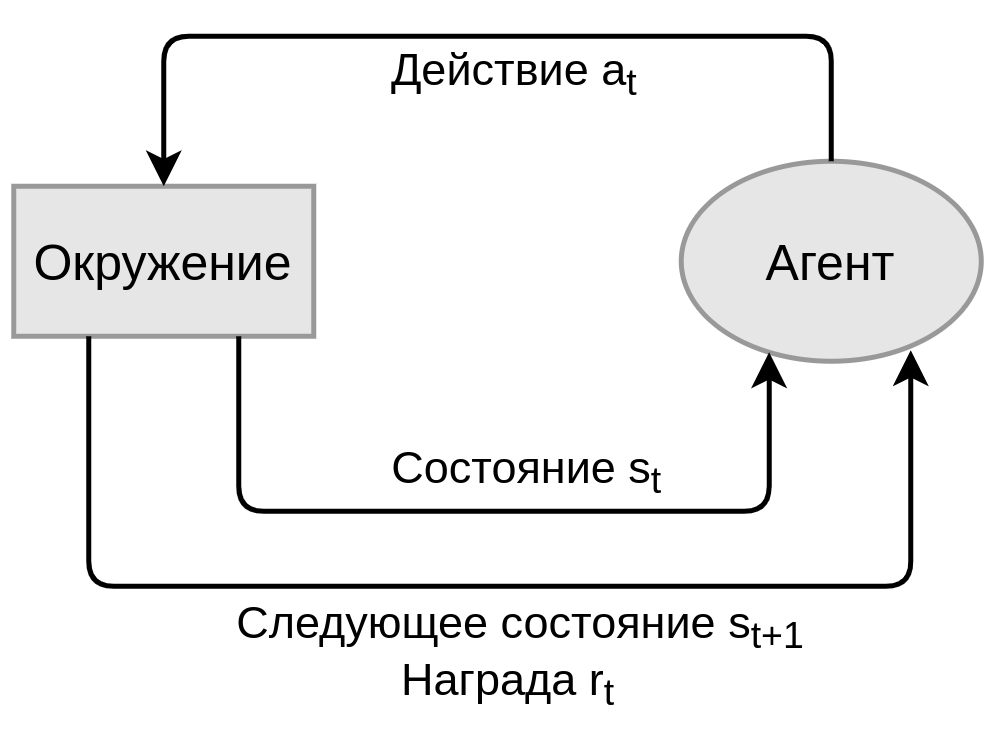
\includegraphics[width=250px]{RLexplanation.png}}
\caption{Один раунд обучения с подкреплением.}
\label{RLexplanation}
\end{figure}

Во всех существующих подходах к тестированию программного обеспечения через взаимодействие с графическим интерфейсом, использующих подход обучения с подкреплением, применяется техника Q-learning. Q-learning -- это самый распространенный и хорошо изученный подход обучения с подкреплением. В нашем случае эта техника используется для поиска оптимального действия для данного состояния мобильного приложения. Различные стратегии и функции наград устанавливают правила, по которым агент должен отдавать предпочтение определенному действию. После выбора и воспроизведения действия среда изменяет свое состояние на новое, и агент получает награду за выполненное действие. На Рис.~\ref{RLexplanation} показана классическая схема одного раунда взаимодействия агента и среды с помощью техники Q-learning:

\begin{enumerate} 

\item Агент получает от окружения состояние $s_t$.

\item Агент выбирает и воспроизводит действие $a_t \in A(s_t)$, где $A(s_t)$ -- множество доступных действий в состоянии $s_t$.

\item Окружение рассчитывает значение функции награды $R(s_t, a_t)$ исходя из состояния $s_t$ и выбранного действия в этом состоянии $a_t$.

\item Окружение рассчитывает новое состояние $s_{t+1}$ исходя из состояния $s_t$ и выбранного действия в этом состоянии $a_t$.

\item Агент получает значение награды $r_t$ и переходит в состояние $s_{t+1}$.

\end{enumerate}

Таким образом, цель агента полностью описывается с помощью функции награды. Поэтому в задачах обучения с подкреплением важно подобрать такую функцию награды, которая будет максимально соответствовать поставленной цели.

За выбор определенного действия в текущем состоянии отвечают так называемые Q-значения. Каждой паре $(s_t, a_t)$ соответствует свое Q-значение, которое описывает потенциальную суммарную награду, которую может получить агент, выбрав действие $a_t$ в состоянии $s_t$. Совокупность всех таких пар описывает Q-таблицу. Таким образом, выбор действия агентом, сводится к тому, чтобы найти максимальное Q-значение в текущем состоянии.

Обучение же модели состоит в том, чтобы подобрать такие Q-значения, которые будут близко описывать потенциальную суммарную награду за выполнение определенного действия. Уравнение, которым описывается обновление Q-значений после получения награды выглядит следующим образом

\begin{equation}
\label{eq_qlearning} 
{\displaystyle
Q(s_t, a_t) = R(s_t, a_t) + \gamma \max_{a_{t+1}}{Q(s_{t+1}, a_{t+1})} ,
}
\end{equation}
где $R(s_t, a_t)$ -- функция награды, $\gamma$ -- фактор дисконтирования, описывающий баланс между немедленной наградой и наградой за будущие действия. Таким образом, за большое число итераций Q-таблица стабилизируется и будет отражать реальную награду за каждое действие.


\subsection{Информация об окружении для тестирования}

Перед тем, как рассматривать конкретные алгоритмы и их реализации, нужно понимать как происходит взаимодействие с устройством. В качестве устройства во всех экспериментах будет выступать официальный эмулятор операционной системы Android. Удобным инструментом для программного взаимодействия с телефоном является утилита командной строки Android Debug Bridge (adb). Именно ее использует DroidBot~\cite{li2017droidbot} для взаимодействия с подключенным устройством. Все реализованные в работе алгоритмы работают на основе генератора тестов DroidBot. Он удобен тем, что может взаимодействовать с приложениями без модификации системы и самого приложения. Это делает DroidBot совместимым со всеми устройствами и приложениями. Также он предоставляет возможность подключать собственные стратегии тестирования, что актуально для этой работы. Еще одна причина, по которой был выбран этот инструмент -- подробный отчет о тестировании, из которого можно получить нужные метрики.

\begin{figure}[h]
\center{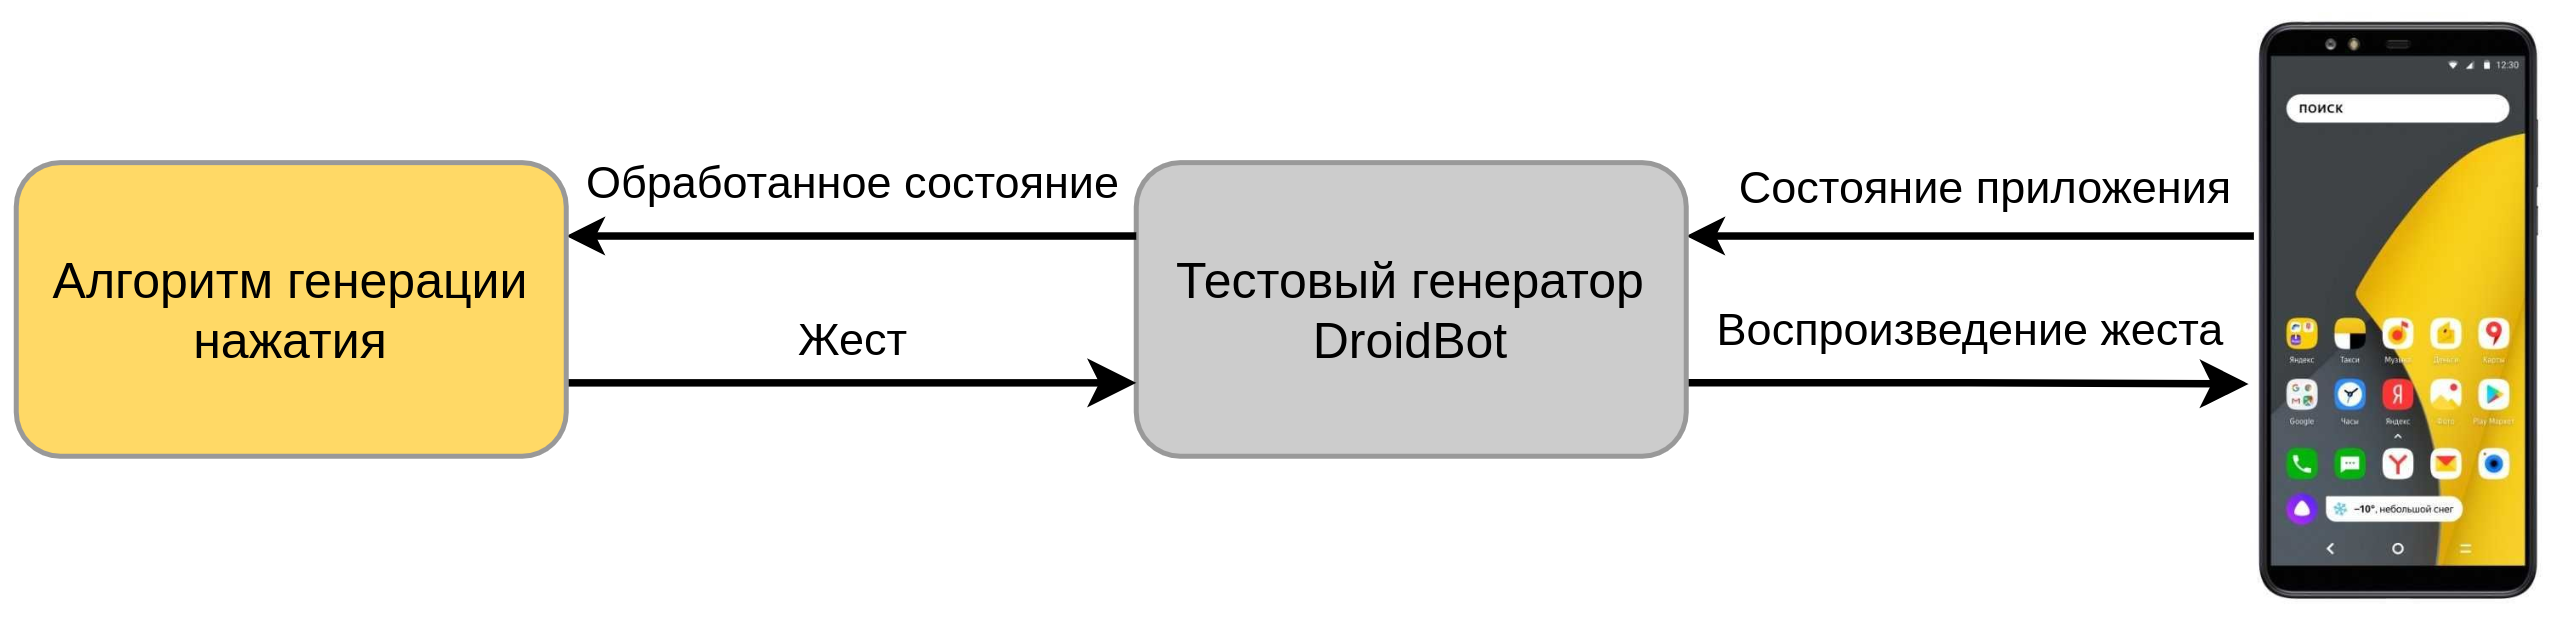
\includegraphics[width=460px]{InteractionScheme.png}}
\caption{Цикл взаимодействия устройства, тестового генератора DroidBot и алгоритма генерации нажатий.}
\label{InteractionScheme}
\end{figure}

Для лучшего понимания процесса тестирования, весь цикл взаимодействия тестового генератора DroidBot и алгоритма генерации нажатий с устройством представлен на Рис.~\ref{InteractionScheme}. Тестовый генератор способен получать текущее состояние приложения от устройства и воспроизводить нажатия на экране смартфона. Получив состояние от устройства, тестовый генератор обрабатывает его и в удобном виде передает алгоритму генерации нажатий.  Алгоритм генерации нажатий путем взаимодействия с тестовым генератором получает обработанное состояние приложения и генерирует жест для воспроизведения на устройстве. Этот жест воспроизводится путем нажатия в нужную координату экрана, и цикл взаимодействия повторяется.

Как было указано в постановке задачи, в работе используется две метрики из четырех основных, введенных в главе~\ref{sec:Chapter0}. Их числовые значения наиболее информативны и понятны. Они обе сопряжены с понятием состояния приложения. Проблема представления состояния приложения в данной работе решается следующим образом: будем считать, что состояния являются одинаковыми, если список возможных взаимодействий в этих состояниях совпадает. То есть состоянием в этой работе является список возможных взаимодействий в текущий момент времени. Действие в данном состоянии можно описать парой (тип действия, интерактивный элемент). Каждый интерактивный элемент имеет свои типы взаимодействия с ним. Эту информацию предоставляет тестовый генератор DroidBot. Таким образом, в каждый момент времени у нас есть доступ к текущему состоянию и всевозможным взаимодействиям в этом состоянии.

Что касается Активности приложения, то ее тоже можно сопоставлять с некоторым понятием состояния. Отличие состоит в том, что Активность приложения является более обобщенным понятием состояния, которое является единым для всех приложений и описывается классом языка программирования. Несколько состояний в нашем понимании могут находиться в одной Активности. Измерения только Активности приложения может быть недостаточно, так как приложение может содержать только одну Активность и при этом множество состояний. Таким образом, метрика Активности приложения всегда будет ниже метрики состояний, но при этом эти метрики независимы и хорошо отражают степень покрытия приложения при тестировании. Если говорить про две другие метрики, то они не будут рассматриваться в этой работе. Причина отказа от метрики с покрытием кода состоит в том, что тестирование в данной работе проводится по стратегии <<черный ящик>>: без доступа к исходному коду. Отказ от метрики с количеством найденных ошибок связан с тем, что эксперименты для проверки эффективности тестирования проводятся на уже готовых приложениях, количество сбоев в которых крайне мало.

Чем больше типов взаимодействия с экраном смартфона будет поддержано во время тестирования, тем потенциально большего покрытия удастся достичь. Поэтому будем использовать все типы жестов, которые предоставляет интерфейс DroidBot: нажатие, двойное нажатие, удержание, вставка текста, горизонтальная и вертикальная прокрутка, кнопки <<Меню>> и <<Назад>>.

Как и требовалось в постановке, все эксперименты в работе будут проводиться на одной и той же ЭВМ. В нашем случае спецификация ЭВМ следующая: \texttt{Intel(R) Core(TM) i7-8700 CPU @ 3.20GHz, 64 GB RAM, GeForce GTX 1080}.

\subsection{Настройка гиперпараметров}

В этой части работы будет определено два основных параметра для всех алгоритмов: количество запусков и время тестирования. Для проведения всех экспериментов был реализован базовый алгоритм Q-learning~\cite{adamo2018reinforcement}, подробное описание которого будет дано позже.

В некоторых алгоритмах, которые будут рассматриваться в дальнейшем, присутствует элемент случайности. Таким образом, тестирование от запуска к запуску может показывать различные значения метрик. Однако это не единственный источник недетерминированности. Так как запуски проводятся на эмуляторе реального устройства, то его работа может сопровождаться некоторыми зависаниями. В добавок ко всему долгая загрузка страниц приложения, наличие анимации и задержки Android Debug Bridge могут привести к различным результатам одного и того же алгоритма. Степень недетерминированности базового алгоритма можно оценить по Рис.~\ref{indeterminacy}. На нем представлены результаты тестирования шести приложений в виде диаграмм размаха. Хорошо видна необходимость проводить эксперименты по несколько раз и результат усреднять. Для всех дальнейших алгоритмов измерения будут проводиться по пять раз. 

Постановка задачи требовала от алгоритма ограниченности по времени, так как в практических приложениях тестирование должно занимать разумное количество времени. Проведем эксперименты на базовом Q-learning алгоритме для вычисления оптимального времени тестирования. По результатам замеров на шести приложениях (Рис.~\ref{metric_per_time}) можно видеть, что графики зависимости метрик от времени выпуклы вверх. Это означает, что с течением времени эффективность поиска новых состояний уменьшается. Для некоторых приложений есть ощутимая разница между 10 и 15 минутами тестирования, но для большинства это несущественный прирост метрики. В качестве компромисса все дальнейшие эксперименты будут проводиться с ограничением времени 12 минут.

\begin{figure}[h]
\centering
\subfloat[Разброс метрики уникальных состояний.]{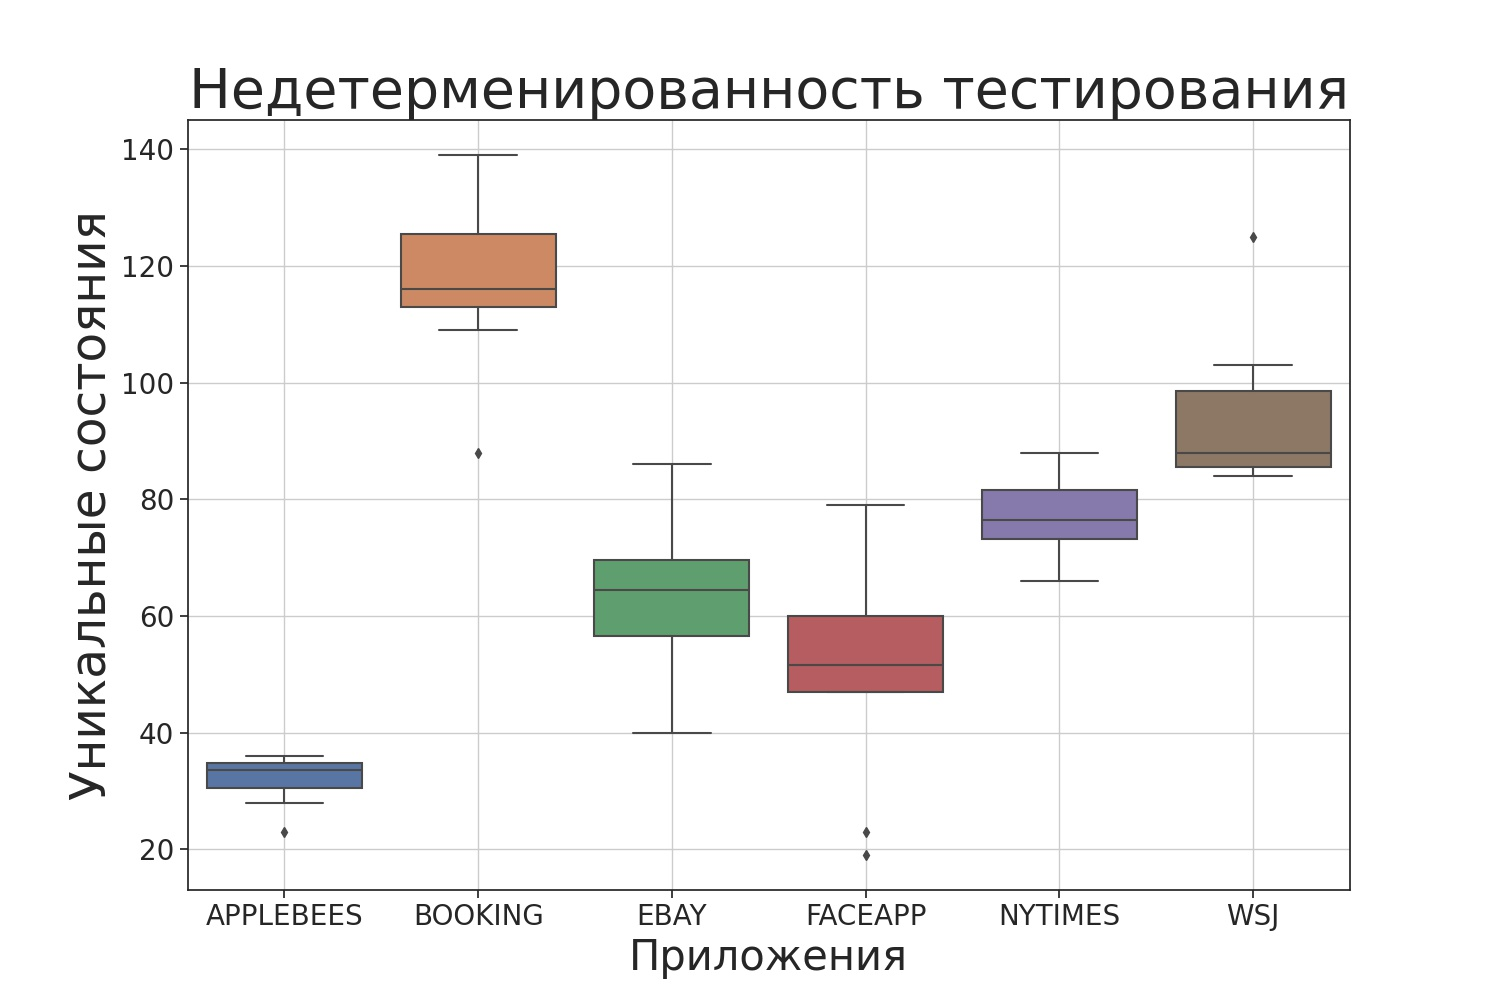
\includegraphics[width=240px]{states_indeterminacy.jpg}} 
\subfloat[Разброс метрики уникальных Активностей.]{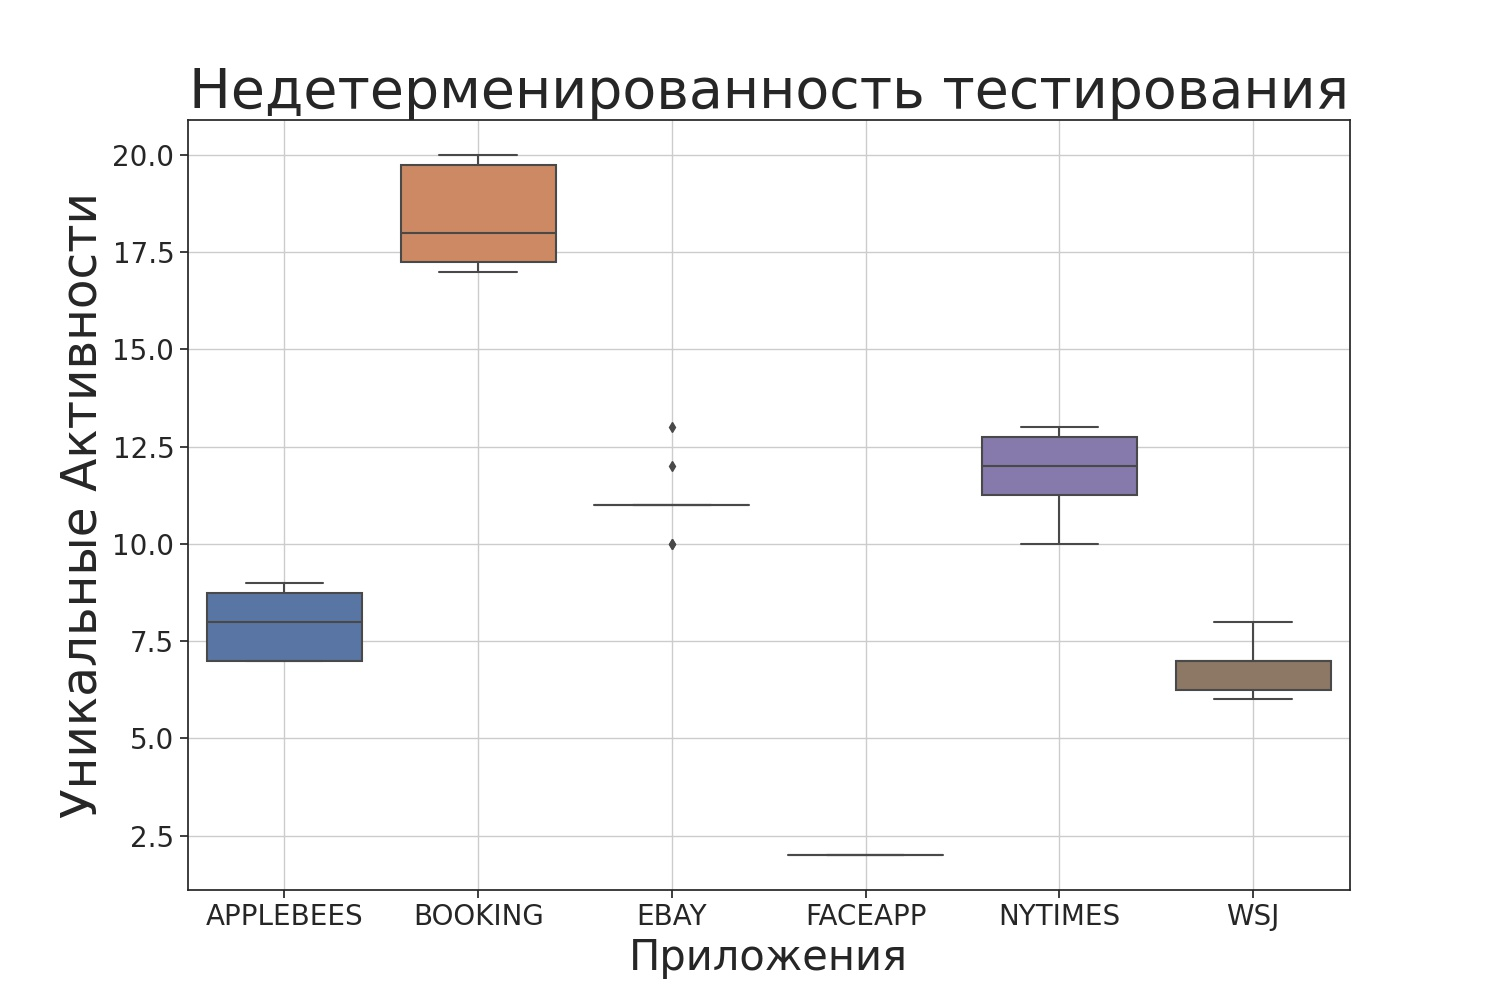
\includegraphics[width=240px]{activities_indeterminacy.jpg}}
\caption{Недетерминированность тестирования.}
\label{indeterminacy}
\end{figure}

\begin{figure}[h]
\centering
\subfloat[Зависимость метрики состояний от времени.]{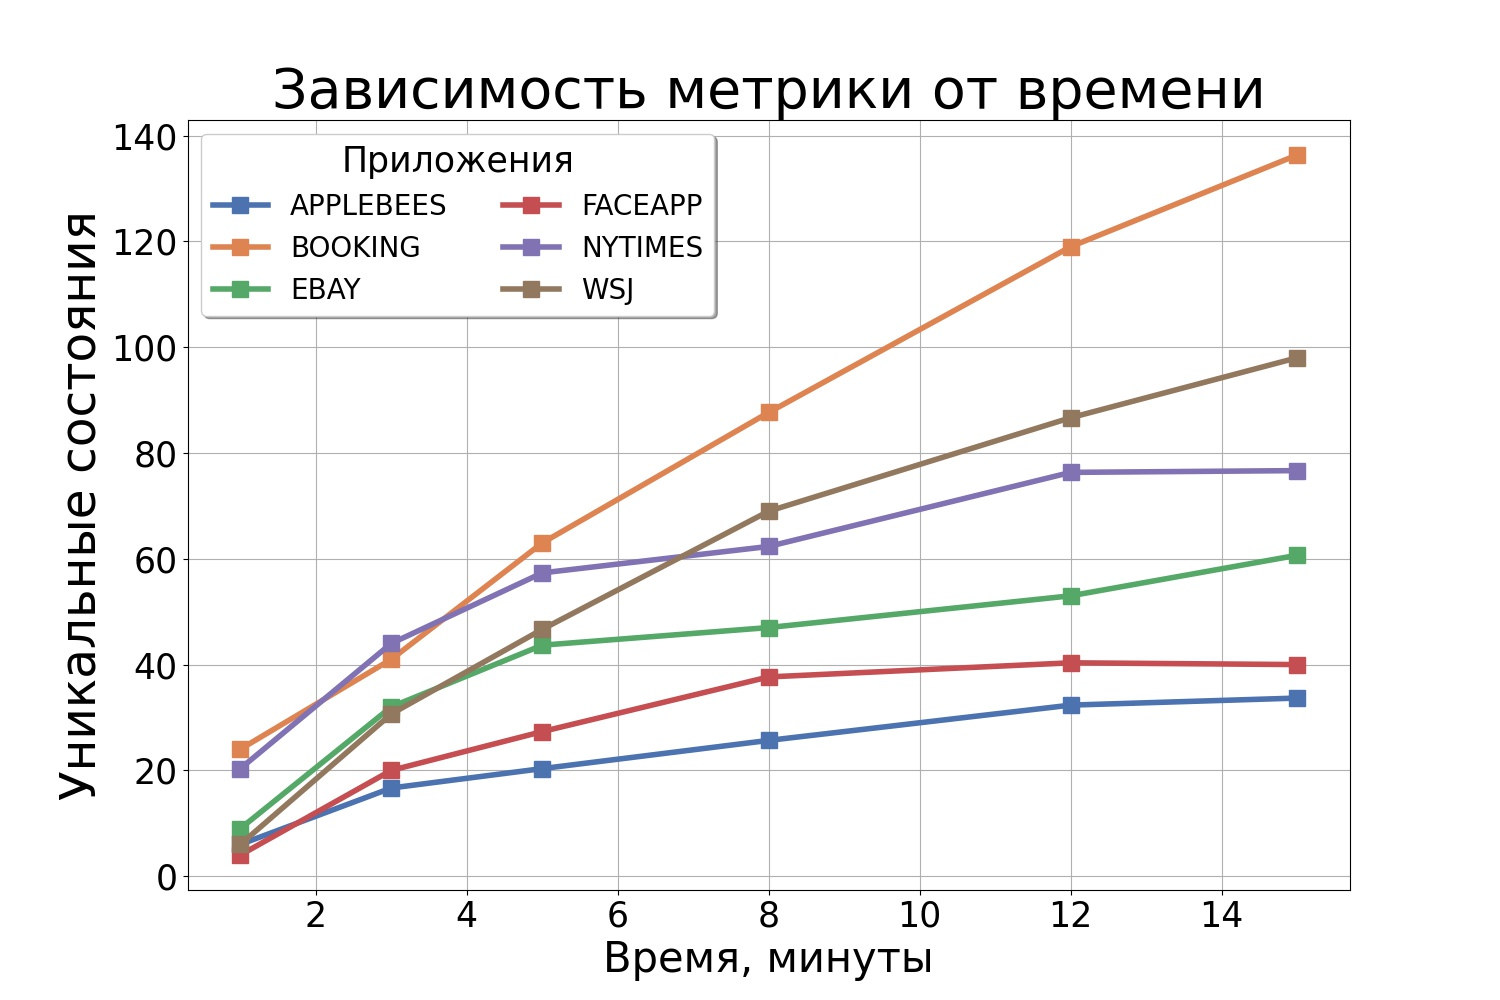
\includegraphics[width=240px]{states_per_time.jpg}} 
\subfloat[Зависимость метрики Активности от времени.]{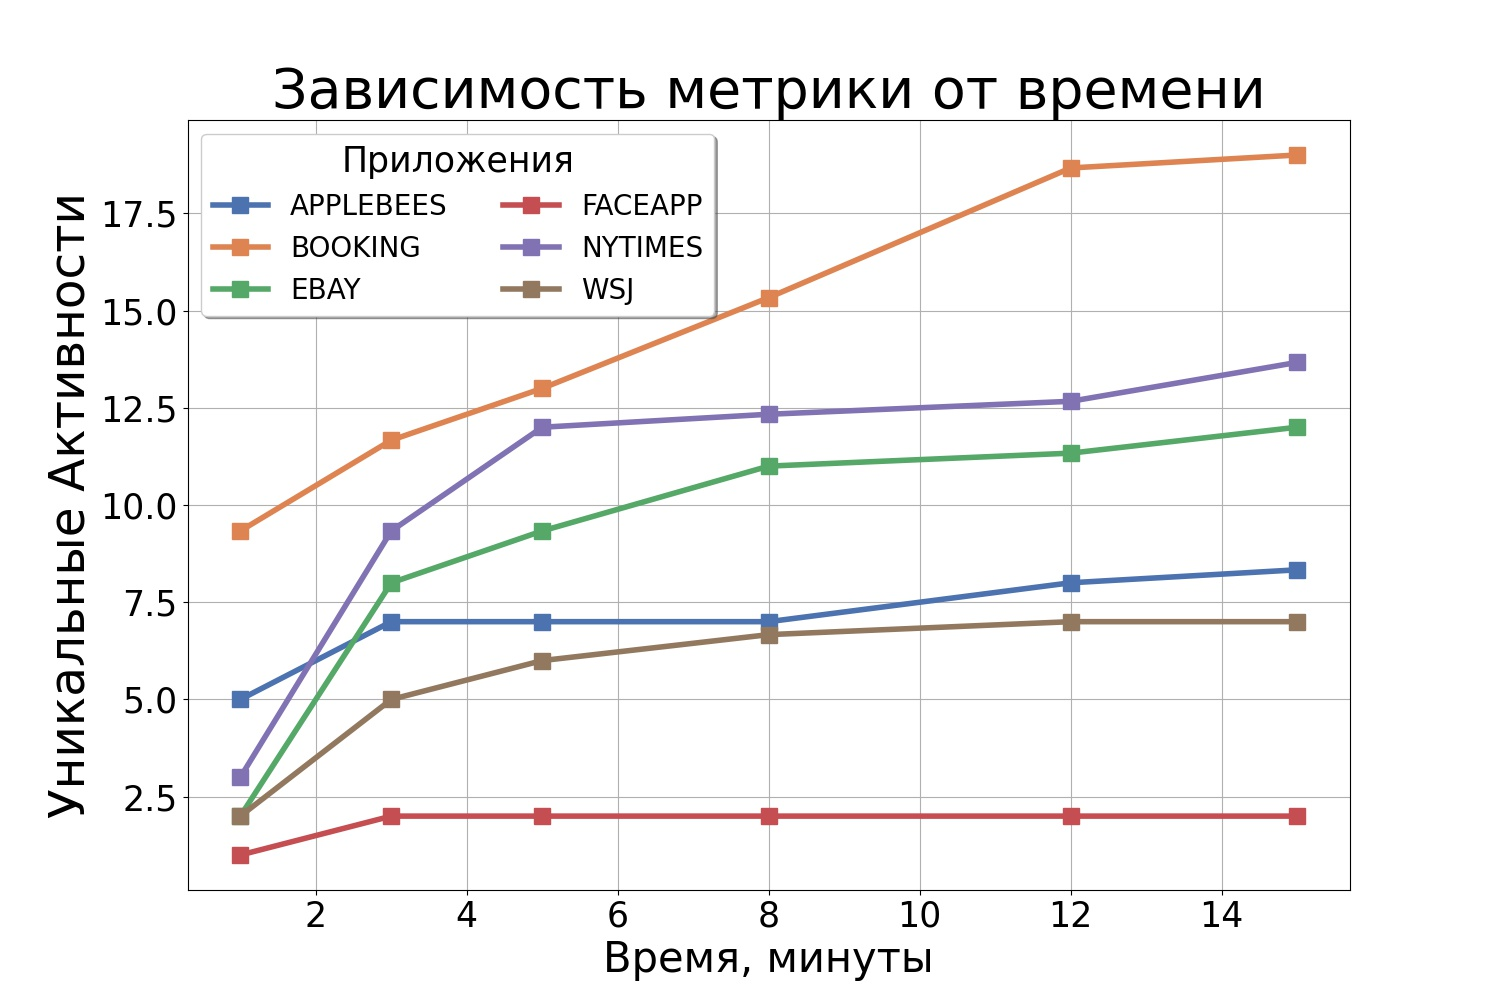
\includegraphics[width=240px]{activities_per_time.jpg}}
\caption{Зависимость метрик от времени.}
\label{metric_per_time}
\end{figure}

\subsection{Приложения}

Чтобы сделать процесс тестирования наиболее честным, возьмем для тестирования приложения различных категорий и степеней сложности. Всего будет использоваться 10 современных приложений: \texttt{Booking}, \texttt{EBAY}, \texttt{The New York Times}, \texttt{Applebee's}, \texttt{FaceApp}, \texttt{The Wall Street Journal}, \texttt{AliExpress}, \texttt{Domino's Pizza}, \texttt{ColorNote}, \texttt{Wikipedia}. В их числе есть как простые приложения с небольшим количеством состояний, так и масштабные приложения с платформы Google Play.

\subsection{Независимые от приложения подходы}

Идеальный инструмент тестирования мобильных приложений -- это инструмент, который способен производить эффективное тестирование для произвольного приложения. Именно в поисках такого инструмента исследование начинается с алгоритмов обучения с подкреплением, которые обучают обобщенную модель, способную взаимодействовать с произвольным приложением. Такой подход связан с рядом упрощений. Например, введение обобщенного состояния и обобщенного действия, которые подходят под все приложения. Обучение таких моделей происходит онлайн (во время тестирования), так как только методом проб и ошибок можно научить Q-learning алгоритмы производить эффективные нажатия.

\subsubsection{Абстрактные состояния}

Первая модель, которая была реализована и внедрена в тестирующую систему DroidBot -- это модель основанная на алгоритме, описанном в~\cite{koroglu2018qbe}. Это классическая техника Q-learning, в которой состояние описывается количеством интерактивных элементов в текущий момент времени, а действие в текущем стоянии описывается лишь типом жеста. Таким образом, модель в зависимости от количества интерактивных элементов в текущем состоянии должна предсказывать тип взаимодействия, приводящий к потенциально новым состояниям.

В качестве функции награды была выбрана величина, равная количеству интерактивных элементов в состоянии, в которое перешло приложение после воспроизведения действия. Эта величина способствует посещению состояний с потенциально большой вариативностью для исследования. Таким образом, алгоритм учится выбирать те действия, которые приводят его к <<богатым>> состояниям. Результаты тестирования этого подхода приведены в Таблице~\ref{app_free_table}.

Представление состояния только количеством интерактивных элементов не может детально описать состояние приложения. В следующем пункте будет рассмотрено альтернативное представление состояния.

\subsubsection{Нейронная сеть}

Для улучшения предыдущего подхода, было решено представлять абстрактное состояние в виде изображения. А именно трехмерного тензора размером $(180, 320, 2)$. Можно заметить, что он представляет из себя две матрицы размера $(180, 320)$. Каждая из двух матриц состоит из нулей и единиц. Единицами на первой матрице выделены интерактивные элементы текущего экрана приложения, на второй -- текстовые элементы. Таким образом удалось ввести общее состояние для всех приложений. Для обработки изображений хорошо зарекомендовали себя сверточные нейронные сети. Именно их и будем использовать для предсказания Q-значений.

В этом подходе сверточная нейронная сеть будет моделировать Q-таблицу. В классическом подходе, Q-таблица должна по паре $(s_t, a_t)$ возвращать Q-значение. Для имитации такого возвращения нейронная сеть будет одновременно получать состояние и действие, а возвращать единственное значение -- Q-значение. Чтобы на вход сверточной нейронной сети передать одновременно состояние и действие, модифицируем вход: будем добавлять к тензору состояния еще один бинарный слой размера $(180, 320)$. Этот слой будет выделять единицами точку прикосновения пользователя. Архитектура нейронной сети (Рис.~\ref{neural_network}) была выбрана небольшая, так как данных для обучения будет немного. 

\begin{figure}[h]
\center{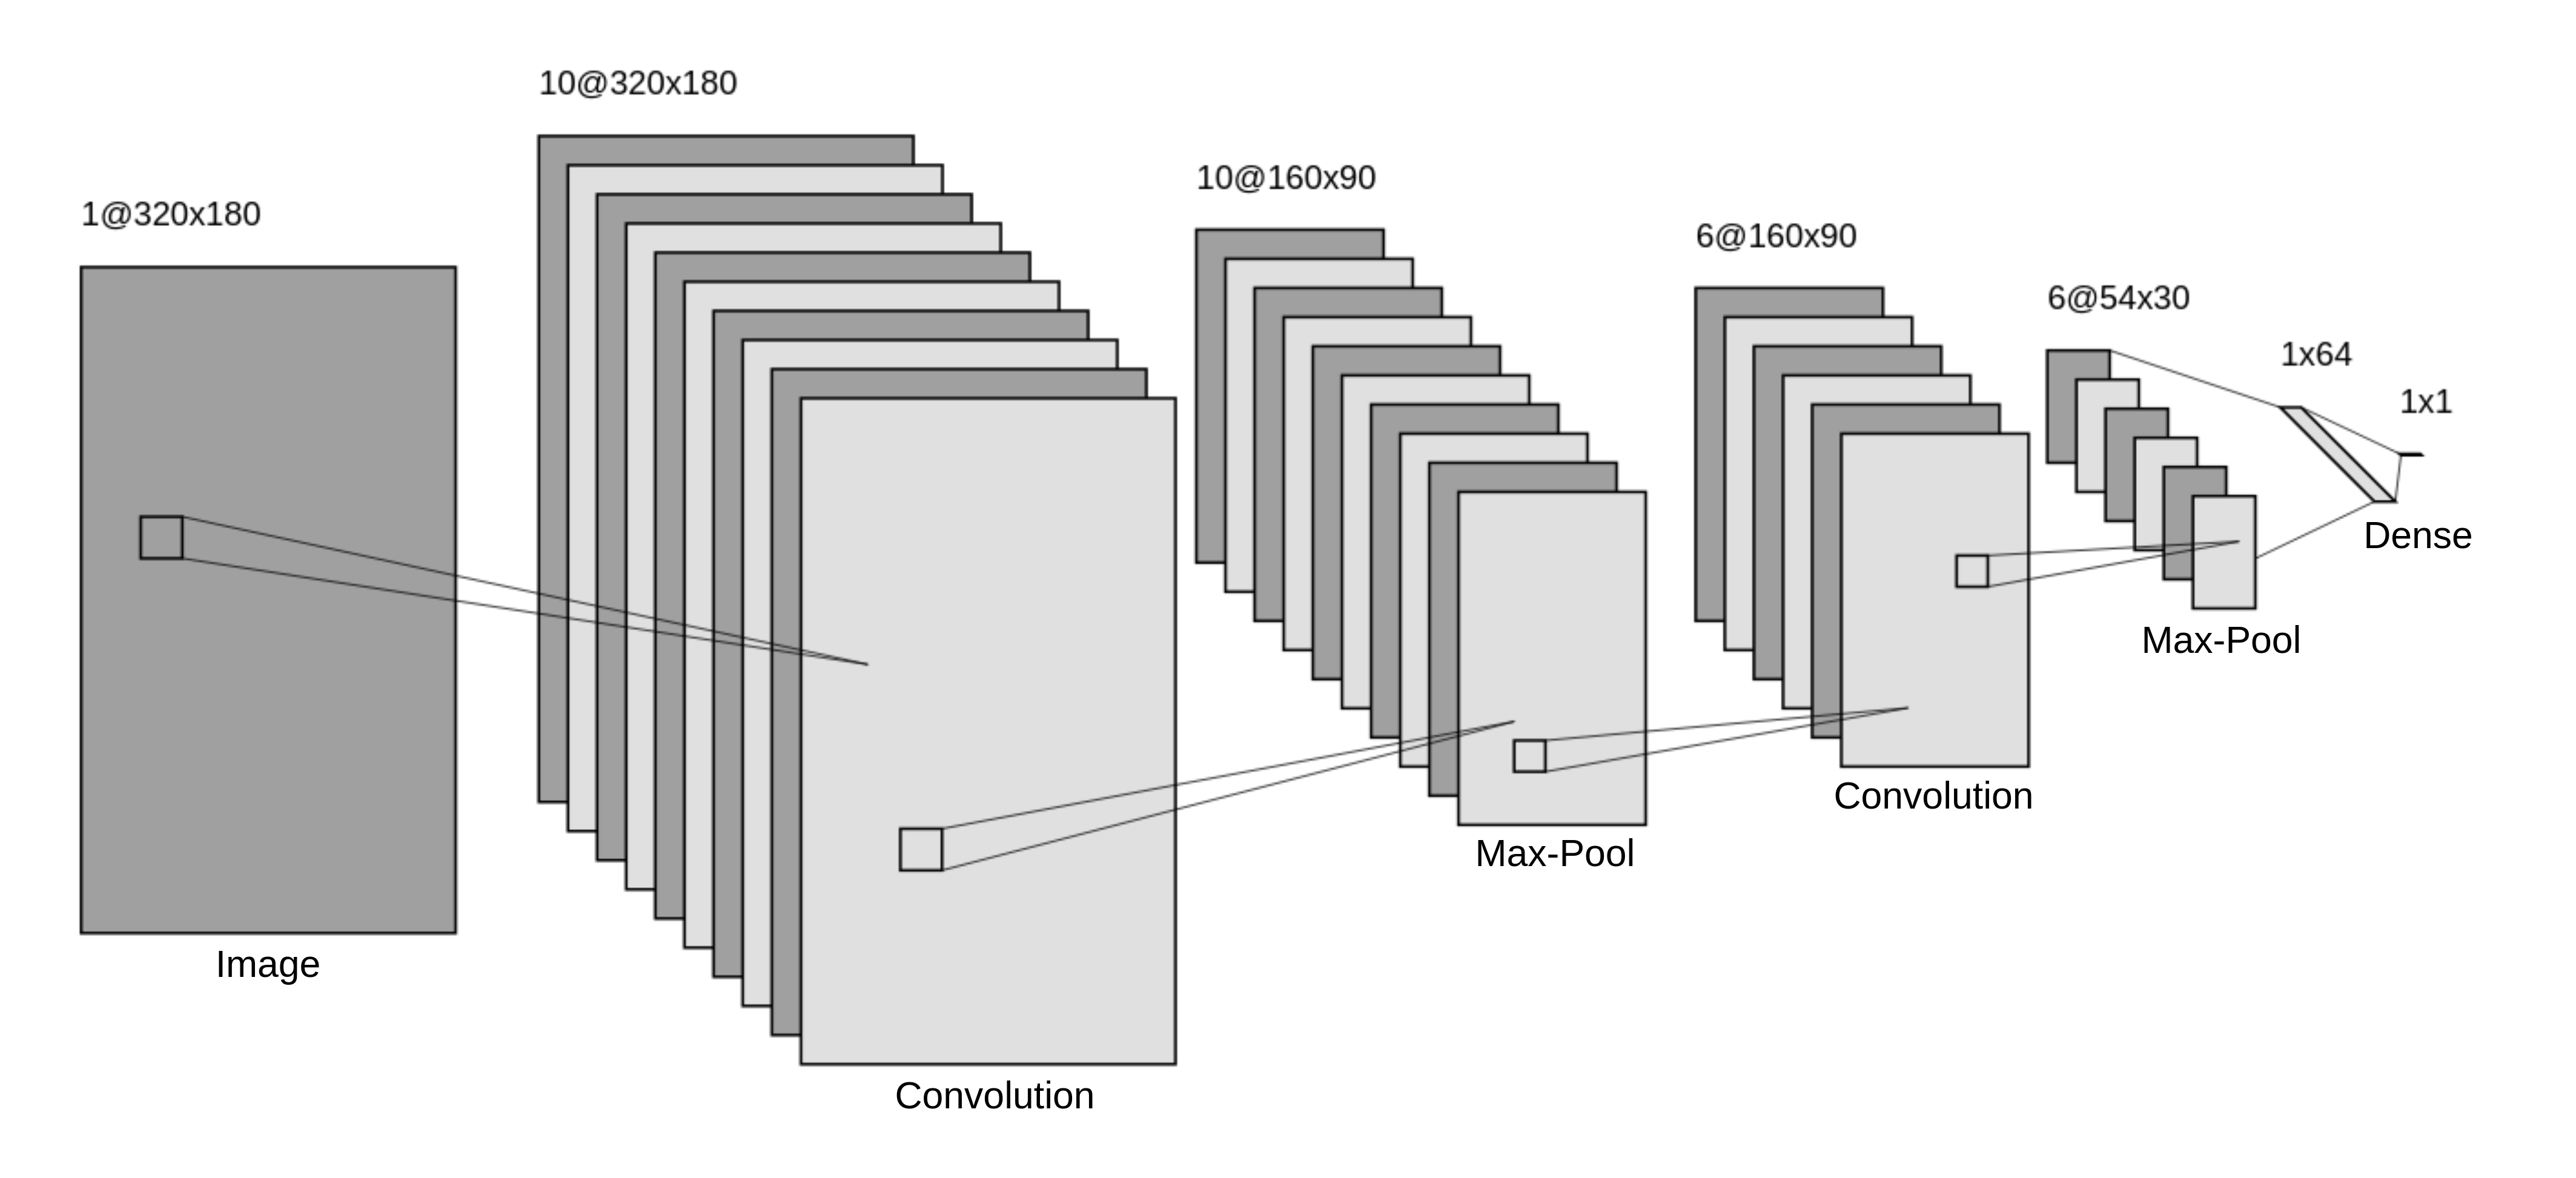
\includegraphics[width=400px]{NeuralNetwork.png}}
\caption{Архитектура нейронной сети для независимого от приложения подхода.}
\label{neural_network}
\end{figure}

Обучение такой сети производится на каждой итерации взаимодействия. Небольшие наборы данных, собранные на всех предыдущих итерациях, постепенно обновляют веса модели и формируют нужную стратегию. Функция награды точно такая же, как и в предыдущем пункте: способствующая более широкому исследованию.

Результаты тестирования этой стратегии приведены в Таблице~\ref{app_free_table}. Для большей наглядности результаты первых двух подходов представлены на Рис.~\ref{app_free_picture} в виде диаграмм размаха.

\begin{table}[h!]
    \centering
    \begin{tabular}{ | l | *{4}{>{\centering\arraybackslash}p{70} |}}
        \hline
        Приложения & \multicolumn{2}{c|}{Абстрактные состояния} & \multicolumn{2}{c|}{Нейронная сеть} \\
        \hline
        ALIEXPRESS &
        \textbf{25} &
        9 & 
        24 & 
        \textbf{12} \\
        \hline
        APPLEBEES &
        \textbf{30} &
        \textbf{7} & 
        23 & 
        \textbf{7} \\
        \hline
        BOOKING &
        \textbf{76} &
        \textbf{18} & 
        45 & 
        13 \\
        \hline
        COLORNOTE &
        52 &
        \textbf{6} & 
        \textbf{81} & 
        \textbf{6} \\
        \hline
        DOMINOS &
        16 &
        \textbf{1} & 
        \textbf{20} & 
        \textbf{1} \\
        \hline
        EBAY &
        \textbf{41} &
        \textbf{8} & 
        24 & 
        6 \\
        \hline
        FACEAPP &
        36 &
        \textbf{2} & 
        \textbf{37} & 
        \textbf{2} \\
        \hline
        NYTIMES &
        \textbf{34} &
        \textbf{6} & 
        27 & 
        \textbf{6} \\
        \hline
        WIKIPEDIA &
        \textbf{118} &
        \textbf{11} & 
        65 & 
        9 \\
        \hline
        WSJ &
        36 &
        7 & 
        \textbf{53} & 
        \textbf{8} \\
        \hline
    \end{tabular}
    \caption{Независимые от приложения стратегии тестирования. Метрика слева -- уникальные состояния, справа -- уникальные Активности.}
    \label{app_free_table}
\end{table}

\begin{figure}[h!]
\centering
\subfloat[Метрика: уникальные состояния.]{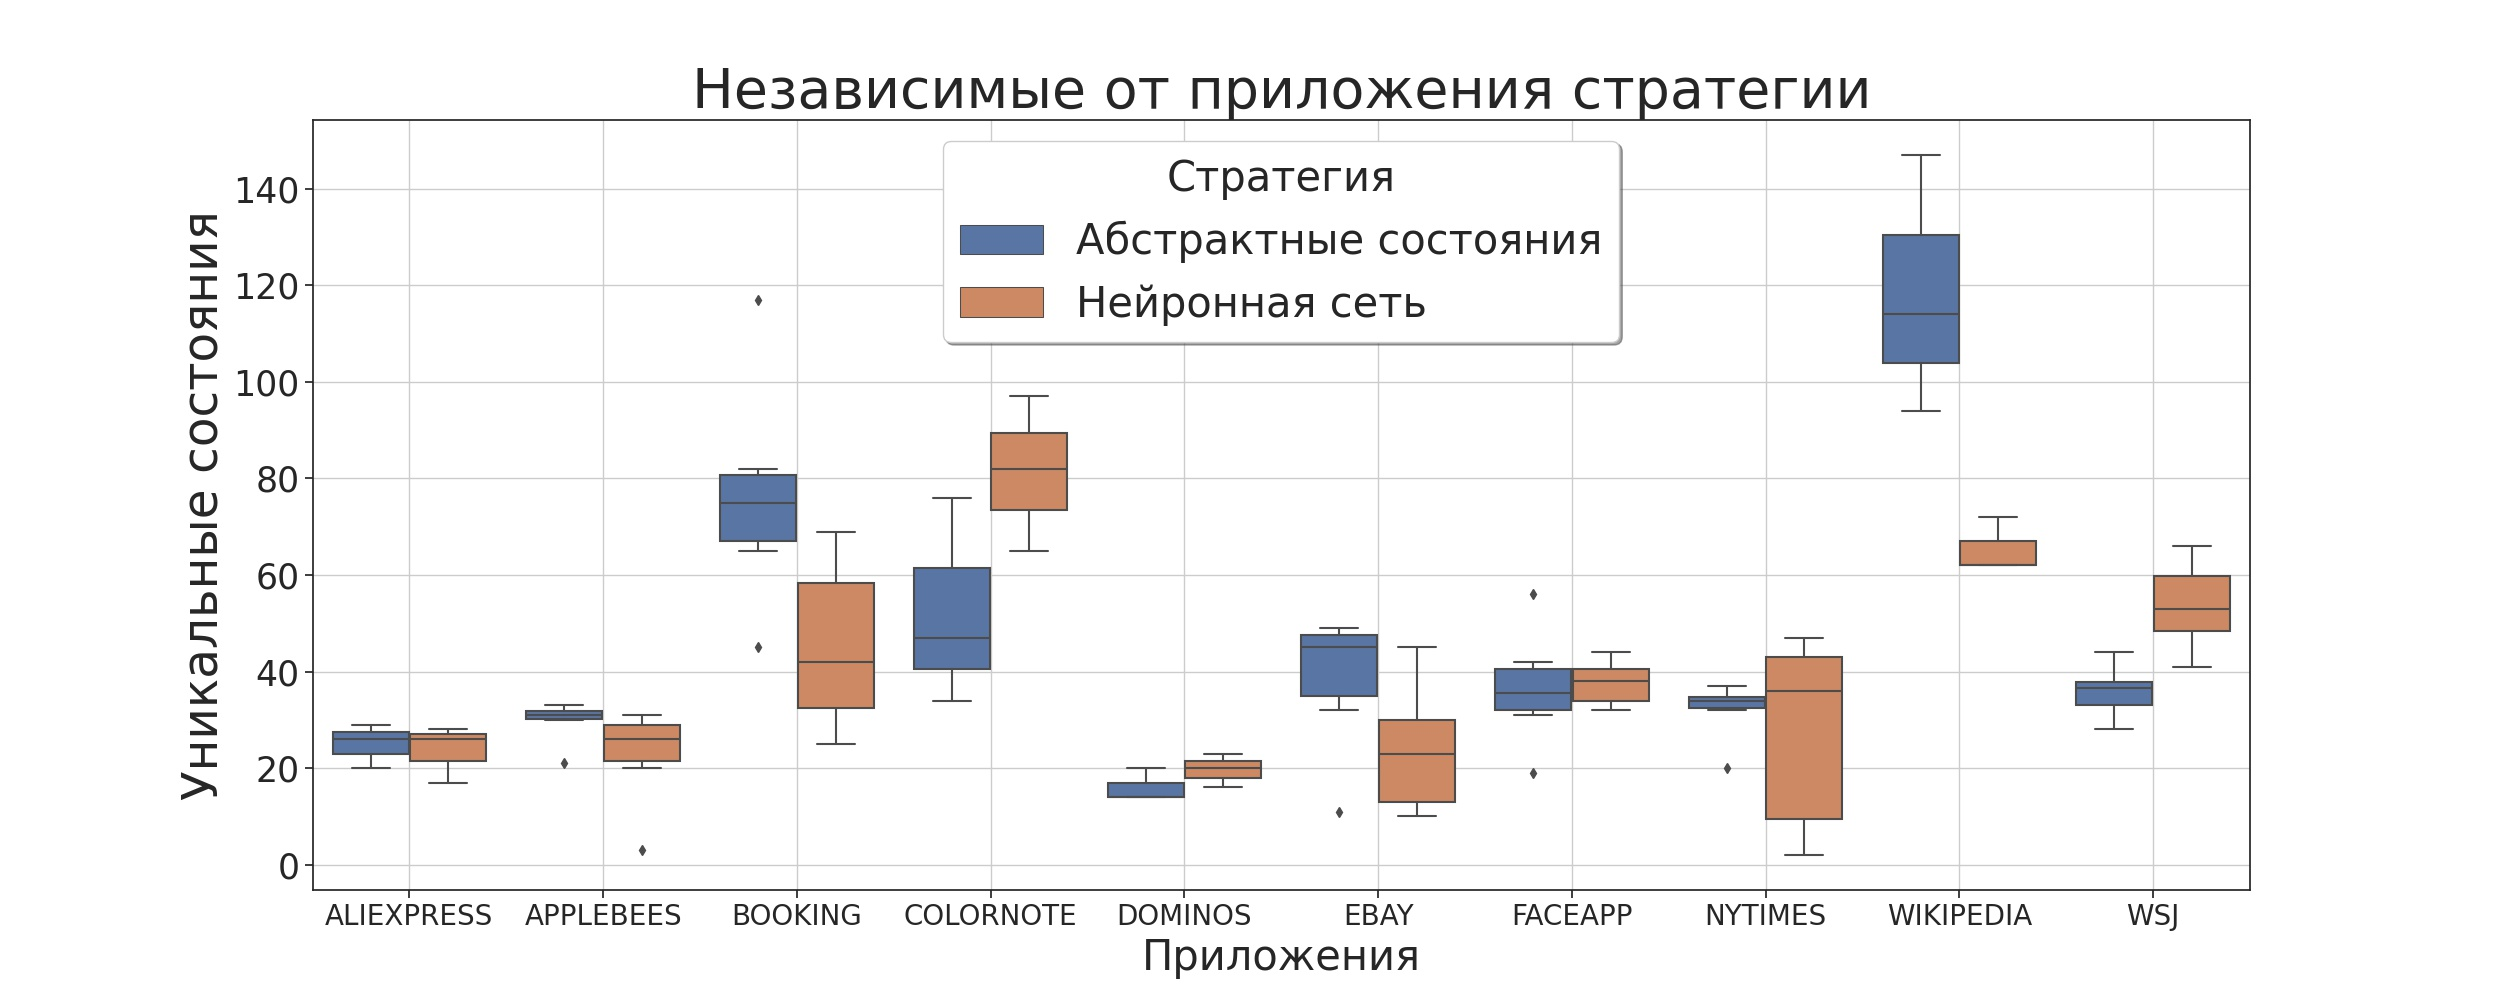
\includegraphics[width=430px]{states_app_free.jpg}} \\
\subfloat[Метрика: уникальные Активности.]{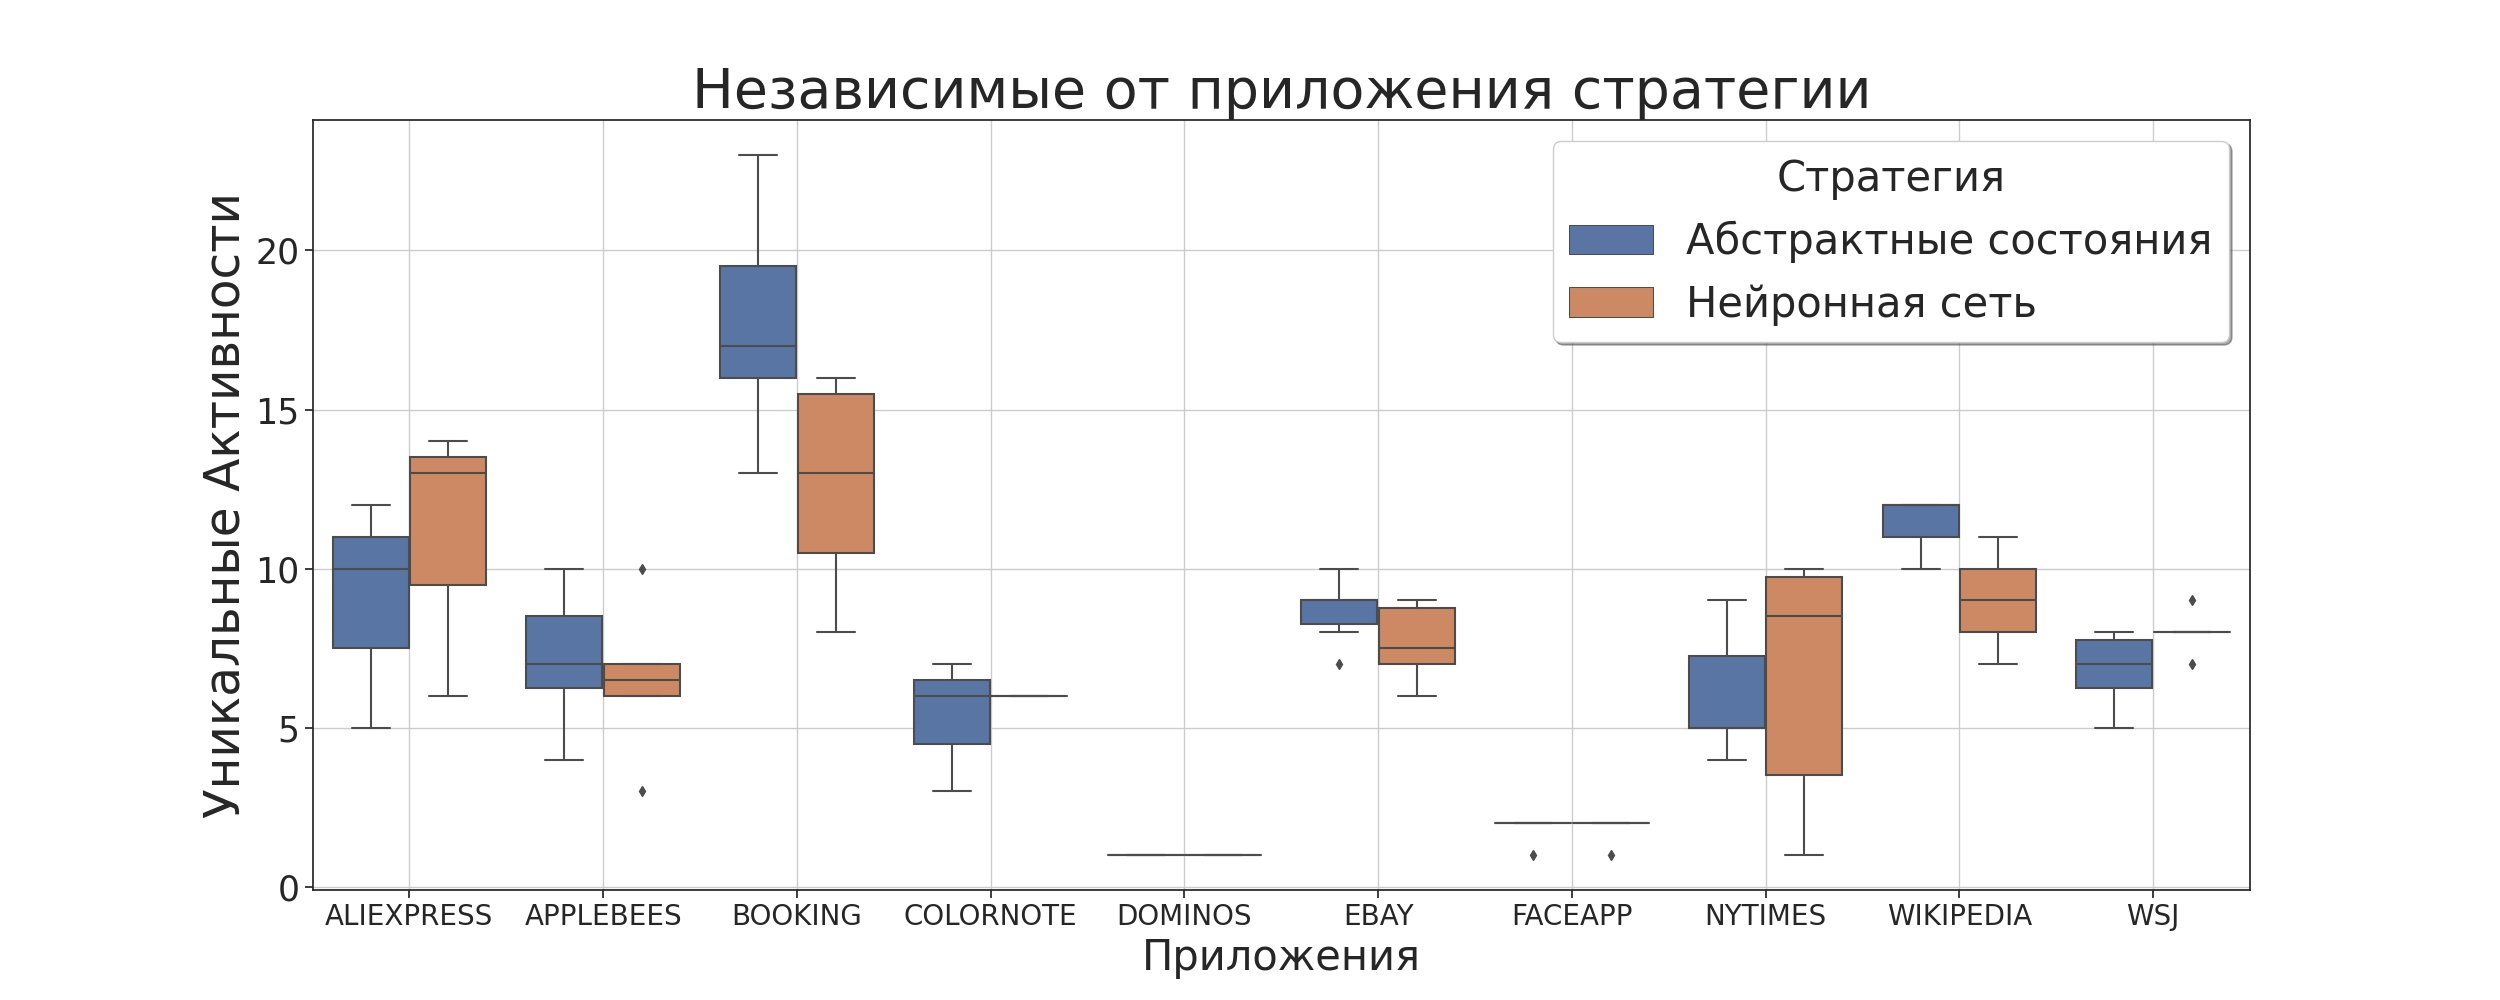
\includegraphics[width=430px]{activities_app_free.jpg}}
\caption{Независимые от приложения стратегии тестирования.}
\label{app_free_picture}
\end{figure}

Можно заметить, что на 6 из 10 приложениях подход основанный на использовании нейронной сети уступает классическому алгоритму Q-learning. В результате анализа было выяснено, что за время, отведенное под тестирование (12 минут), алгоритм не успевает собрать достаточно данных для обучения, и тем самым нейронная сеть не успевает выучить нужные шаблоны тестирования. Однако, на четырех приложениях нейронная сеть оказалась лучше. Это связано с тем, что на этих приложениях визуальная составляющая состояний не сильно изменяется при переходе в разные Активности. Можно заметить, что все четыре приложения имеют малое количество уникальных Активностей, что говорит о низкой вариативности структуры графического интерфейса. Это облегчает обучение нейронной сети.

\subsection{Зависимые от приложения подходы}

Повышения производительности тестирования приложения можно добиться, если перейти от идеи тестирования произвольного приложения к тестированию конкретного приложения. С целью улучшения метрик качества, перейдем к рассмотрению моделей, способных тестировать только то приложение, под которое они обучаются. Идея этих методов в том, что состояния и действия в Q-таблице теперь будут означать конкретные состояния и действия текущего приложения. Такая персонализация позволит обучить модель с учетом тонкостей приложения.

Как было сказано ранее, функция награды полностью определяет цель тестирования. Рассмотрим несколько функций наград, способных увеличить эффективность тестирования приложения.

\subsubsection{Награда: частота нажатий}\label{events_count}

Наиболее простым Q-learning подходом для этих целей является модель~\cite{adamo2018reinforcement}. У этого метода функция награды содержит только частоту нажатия определенного действия. Суть метода в том, что изначально Q-значение за любое действие в любом состоянии равно константе. Однако при очередном выборе действия Q-значение за это действие корректируется: уменьшается пропорционально количеству выполнений этого действия в текущем состоянии. Таким образом, уже протестированные действия текущего состояния будут иметь меньшее Q-значение. Q-значения в этом подходе корректируется согласно формуле~(\ref{eq_qlearning}). Функция награды в этом подходе выглядит следующим образом

\begin{equation}
\label{eq_reward}
{\displaystyle
R(s_t, a_t) = \frac{1}{count(s_t, a_t)} ,
}
\end{equation}
где $count(s_t, a_t)$ -- количество раз, которое действие $a_t$ воспроизводилось в состоянии $s_t$. Такой подход будет повторно посещать состояние только в том случае, если он уже посетил все оставшиеся состояния. Результаты тестирования этой стратегии приведены в Таблице~\ref{app_based_table}.

Исходя из формулы~(\ref{eq_reward}) можно заметить, что такой выбор функции награды и обновления Q-значения -- далекий от интеллектуальности подход. Действительно, функция награды зависит только от количества нажатий на интерактивный элемент текущего состояния, что неизбежно приводит к обычному обходу графа состояний. Единственный момент, который отличает эту систему от стандартного обхода -- различные значения $\gamma$ для разных состояний. В этом и следующих подходах фактор дисконтирования $\gamma$ формируется согласно следующей формуле

$$
\gamma = 0.9 e^{\displaystyle{-0.1 |events(s_{t+1})|}} ,
$$
где $events(s_{t+1})$ -- все возможные взаимодействия в состоянии $s_{t+1}$. Такое определение $\gamma$ обоснованно интуитивным предположением о том, что для состояний с меньшим количеством интерактивных элементов нужно отдавать предпочтение будущим наградам. Однако фактор дисконтирования влияет только на степень учета будущих наград. Для увеличения эффективности необходимо усовершенствовать функцию награды. Будем использовать некоторые эвристические предположения для дальнейшего улучшения метрик.

\begin{table}[h]
    \centering
    \begin{tabular}{ | l | *{8}{>{\centering\arraybackslash}p{37}|}}
        \hline
        Приложения & 
        \multicolumn{2}{>{\centering\arraybackslash}p{74}|}{Обратная частота нажатий} & 
        \multicolumn{2}{>{\centering\arraybackslash}p{74}|}{Кол-во интерактивных элементов} &
        \multicolumn{2}{>{\centering\arraybackslash}p{74}|}{Обратное кол-во инт. элементов} &
        \multicolumn{2}{>{\centering\arraybackslash}p{74}|}{Расстояние между состояниями} \\
        \hline
        ALIEXPRESS &
        \textbf{37} &
        \textbf{11} & 
        34 & 
        10 &
        32 &
        9 &
        30 &
        9 \\
        \hline
        APPLEBEES &
        32 &
        7 & 
        30 & 
        7 &
        \textbf{34} &
        \textbf{8} &
        32 &
        7 \\
        \hline
        BOOKING &
        \textbf{116} &
        \textbf{18} & 
        85 & 
        \textbf{18} &
        85 &
        16 &
        86 &
        16 \\
        \hline
        COLORNOTE &
        142 &
        5 & 
        153 & 
        \textbf{6} &
        \textbf{183} &
        5 &
        164 &
        5 \\
        \hline
        DOMINOS &
        \textbf{35} &
        \textbf{1} & 
        34 & 
        \textbf{1} &
        30 &
        \textbf{1} &
        30 &
        \textbf{1} \\
        \hline
        EBAY &
        \textbf{67} &
        \textbf{11} & 
        45 & 
        10 &
        40 &
        \textbf{11} &
        46 &
        \textbf{11} \\
        \hline
        FACEAPP &
        \textbf{54} &
        \textbf{2} & 
        48 & 
        \textbf{2} &
        48 &
        \textbf{2} &
        39 &
        \textbf{2} \\
        \hline
        NYTIMES &
        \textbf{77} &
        11 & 
        45 & 
        11 &
        49 &
        \textbf{12} &
        74 &
        11 \\
        \hline
        WIKIPEDIA &
        74 &
        9 & 
        77 & 
        12 &
        \textbf{95} &
        \textbf{14} &
        46 &
        10 \\
        \hline
        WSJ &
        96 &
        7 & 
        \textbf{117} & 
        \textbf{8} &
        85 &
        7 &
        82 &
        6 \\
        \hline
    \end{tabular}
    \caption{Зависимые от приложения стратегии тестирования. Метрика слева -- уникальные состояния, справа -- Активности.}
    \label{app_based_table}
\end{table}

\subsubsection{Награда: количество интерактивных элементов}\label{possible_events}

Чтобы алгоритм стремился научиться открывать больше новых состояний, ему нужно давать большую награду за переход в состояния, которые потенциально могут привести к более широкому исследованию. Модифицируем функцию награды таким образом, чтобы алгоритм получал большую награду за переход в состояния с большим числом интерактивных элементов. Это позволит учитывать количество интерактивных элементов не только в долгосрочной перспективе (за счет фактора дисконтирования), но и в мгновенной награде. Функция награды в этом случае будет выглядеть так

$$R(s_t, a_t) = \frac{|events(s_{t+1})|}{count(s_t, a_t)},$$
где $count(s_t, a_t)$ -- количество раз, которое действие $a_t$ воспроизводилось в состоянии $s_t$, $events(s_{t+1})$ -- все возможные взаимодействия в состоянии $s_{t+1}$. Результаты тестирования этой стратегии приведены в Таблице~\ref{app_based_table}.

Можно рассмотреть обратную мотивацию. Посещение состояний с большим количеством интерактивных элементов находится в приоритете для Q-learning алгоритма, так как Q-значение вычисляется с учетом максимума на следующем состоянии. Таким образом, вероятность, что максимум будет больше для состояния с большим количество интерактивных элементов, выше, чем для состояний с малым количеством интерактивных элементов. Следовательно, алгоритм может пропускать такие <<бедные>> состояния. Попробуем исправить эту ситуацию тем, что увеличим награду за посещение состояний с малым количеством интерактивных элементов. Это способствует исследованию граничных состояний перед тем, как заходить в потенциально <<богатые>> состояния. Функция награды выглядит следующим образом 

$$R(s_t, a_t) = \frac{1}{|events(s_{t+1})|count(s_t, a_t)},$$
где $count(s_t, a_t)$ -- количество раз, которое действие $a_t$ воспроизводилось в состоянии $s_t$, $events(s_{t+1})$ -- все возможные взаимодействия в состоянии $s_{t+1}$. Результаты тестирования этой стратегии приведены в Таблице~\ref{app_based_table}.

\subsubsection{Награда: расстояние между состояниями}

Можно рассмотреть еще одну эвристику -- если нажатие на экран приводит к состоянию, близкому к предыдущему (например, открыт выпадающий список), то скорее всего это действие менее ценное, чем то, которое привело бы к кардинально новому состоянию (новой Активности). Состояния приложения можно представлять в виде дерева, в котором интерактивные элементы с их атрибутами находятся в узлах, а вложенные элементы порождают иерархию дерева. Следовательно,  мерой расстояния между состояниями может служить расстояние редактирования графов. Установим это расстояние как функцию награды и проведем измерения эффективности тестирования. Функция награды в этом случае будет выглядеть следующим образом

$$R(s_t, a_t) = \frac{dist(s_t, s_{t+1})}{count(s_t, a_t)},$$
где $count(s_t, a_t)$ -- количество раз, которое действие $a_t$ воспроизводилось в состоянии $s_t$, $dist(s_t, s_{t+1})$ -- расстояние редактирования между графами состояний $s_{t}$ и $s_{t+1}$, которое описывается следующей формулой

$$dist(s_{t},s_{t+1}) = \min_{(e_{1},...,e_{k}) \in \mathcal{P}(s_{t},s_{t+1})} \sum_{i=1}^{k} c(e_{i}) ,$$
где  $\mathcal {P}(s_{t},s_{t+1})$ означает набор преобразования графа $s_{t}$ к графу  $s_{t+1}$, а $c(e)\geqslant 0$ равна стоимости каждой операции преобразования $e$. Стоимость вставки и удаления вершины в этой работе равна единице. Результаты тестирования этой стратегии приведены в Таблице~\ref{app_based_table}.

Для наглядности результаты тестирования всех стратегий, зависящих от приложения, представлены в виде диаграмм размаха на Рис.~\ref{app_based_picture}.


В сравнении результатов стратегий, независимых от приложения (Таблица~\ref{app_free_table}), с результатами последних стратегий (Таблица~\ref{app_based_table}) очевидно превосходство вторых. Несмотря на то, что приложение Wikipedia немного снизило показатели, метрики на остальных приложениях сильно возросли. Как и ожидалось, переход на обучение под конкретное приложение позволил повысить эффективность тестирования.

\begin{figure}[h!]
\centering
\subfloat[Метрика: состояния.]{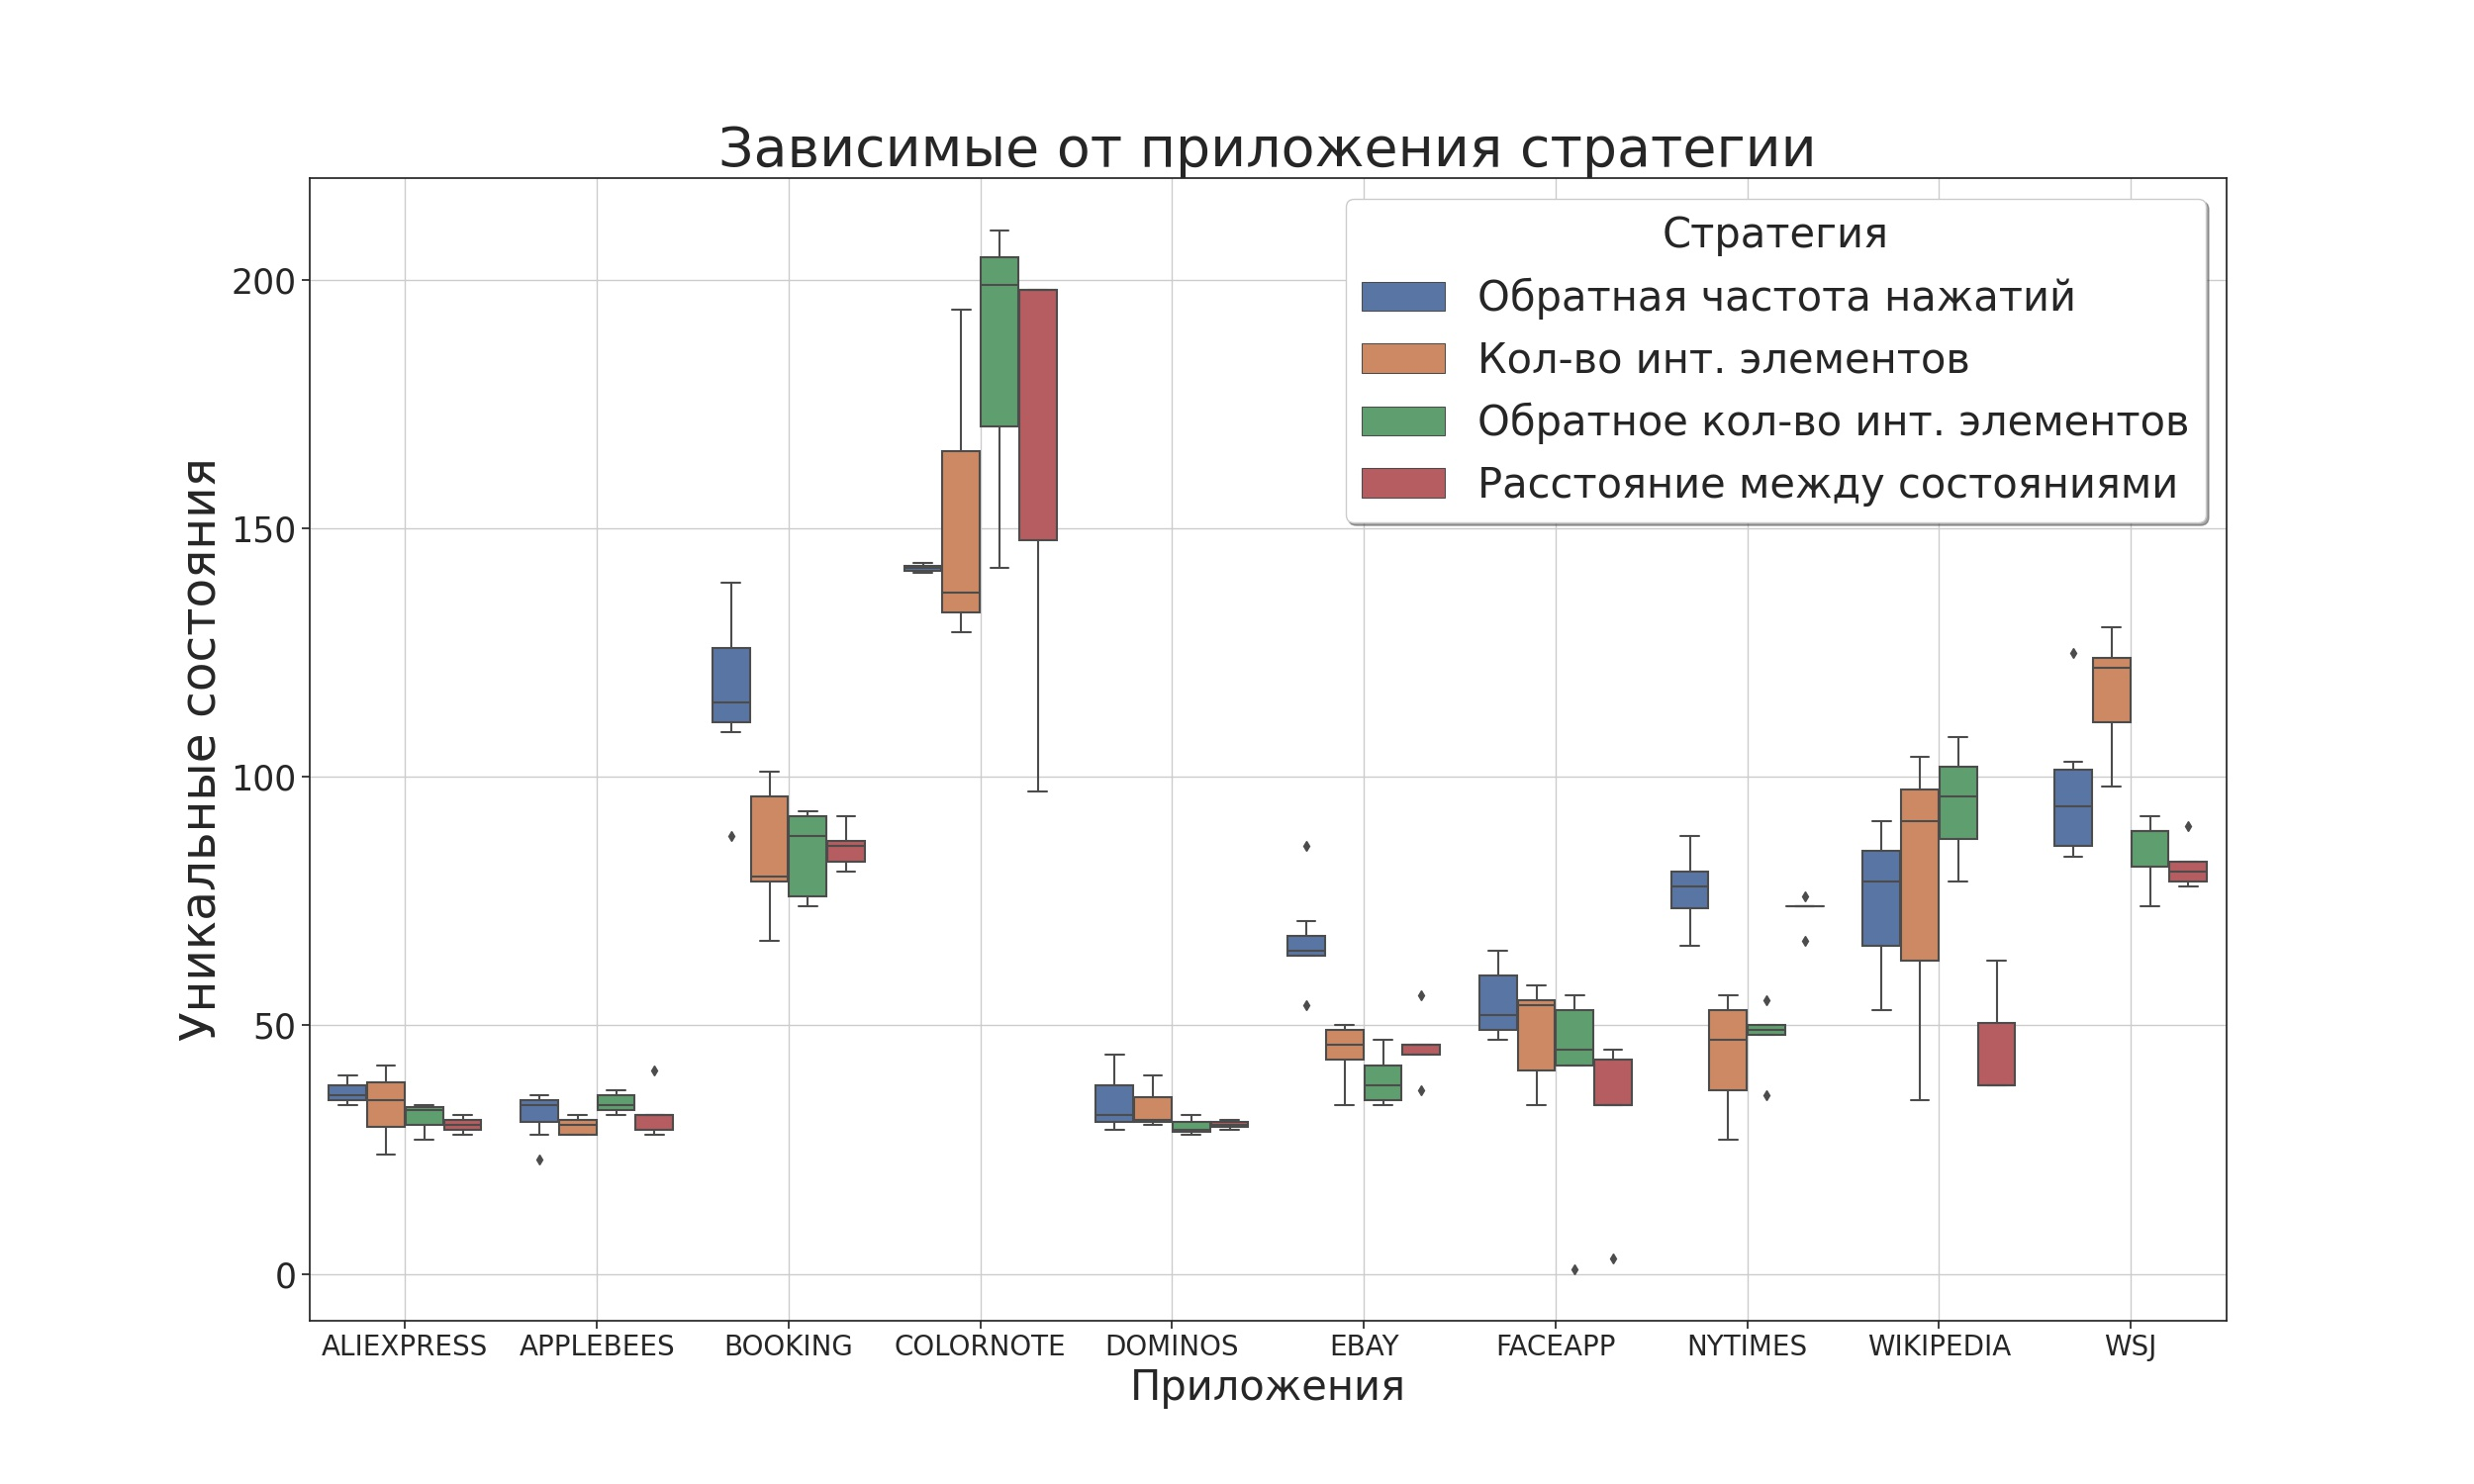
\includegraphics[width=400px]{states_app_based.jpg}} \\
\subfloat[Метрика: Активности.]{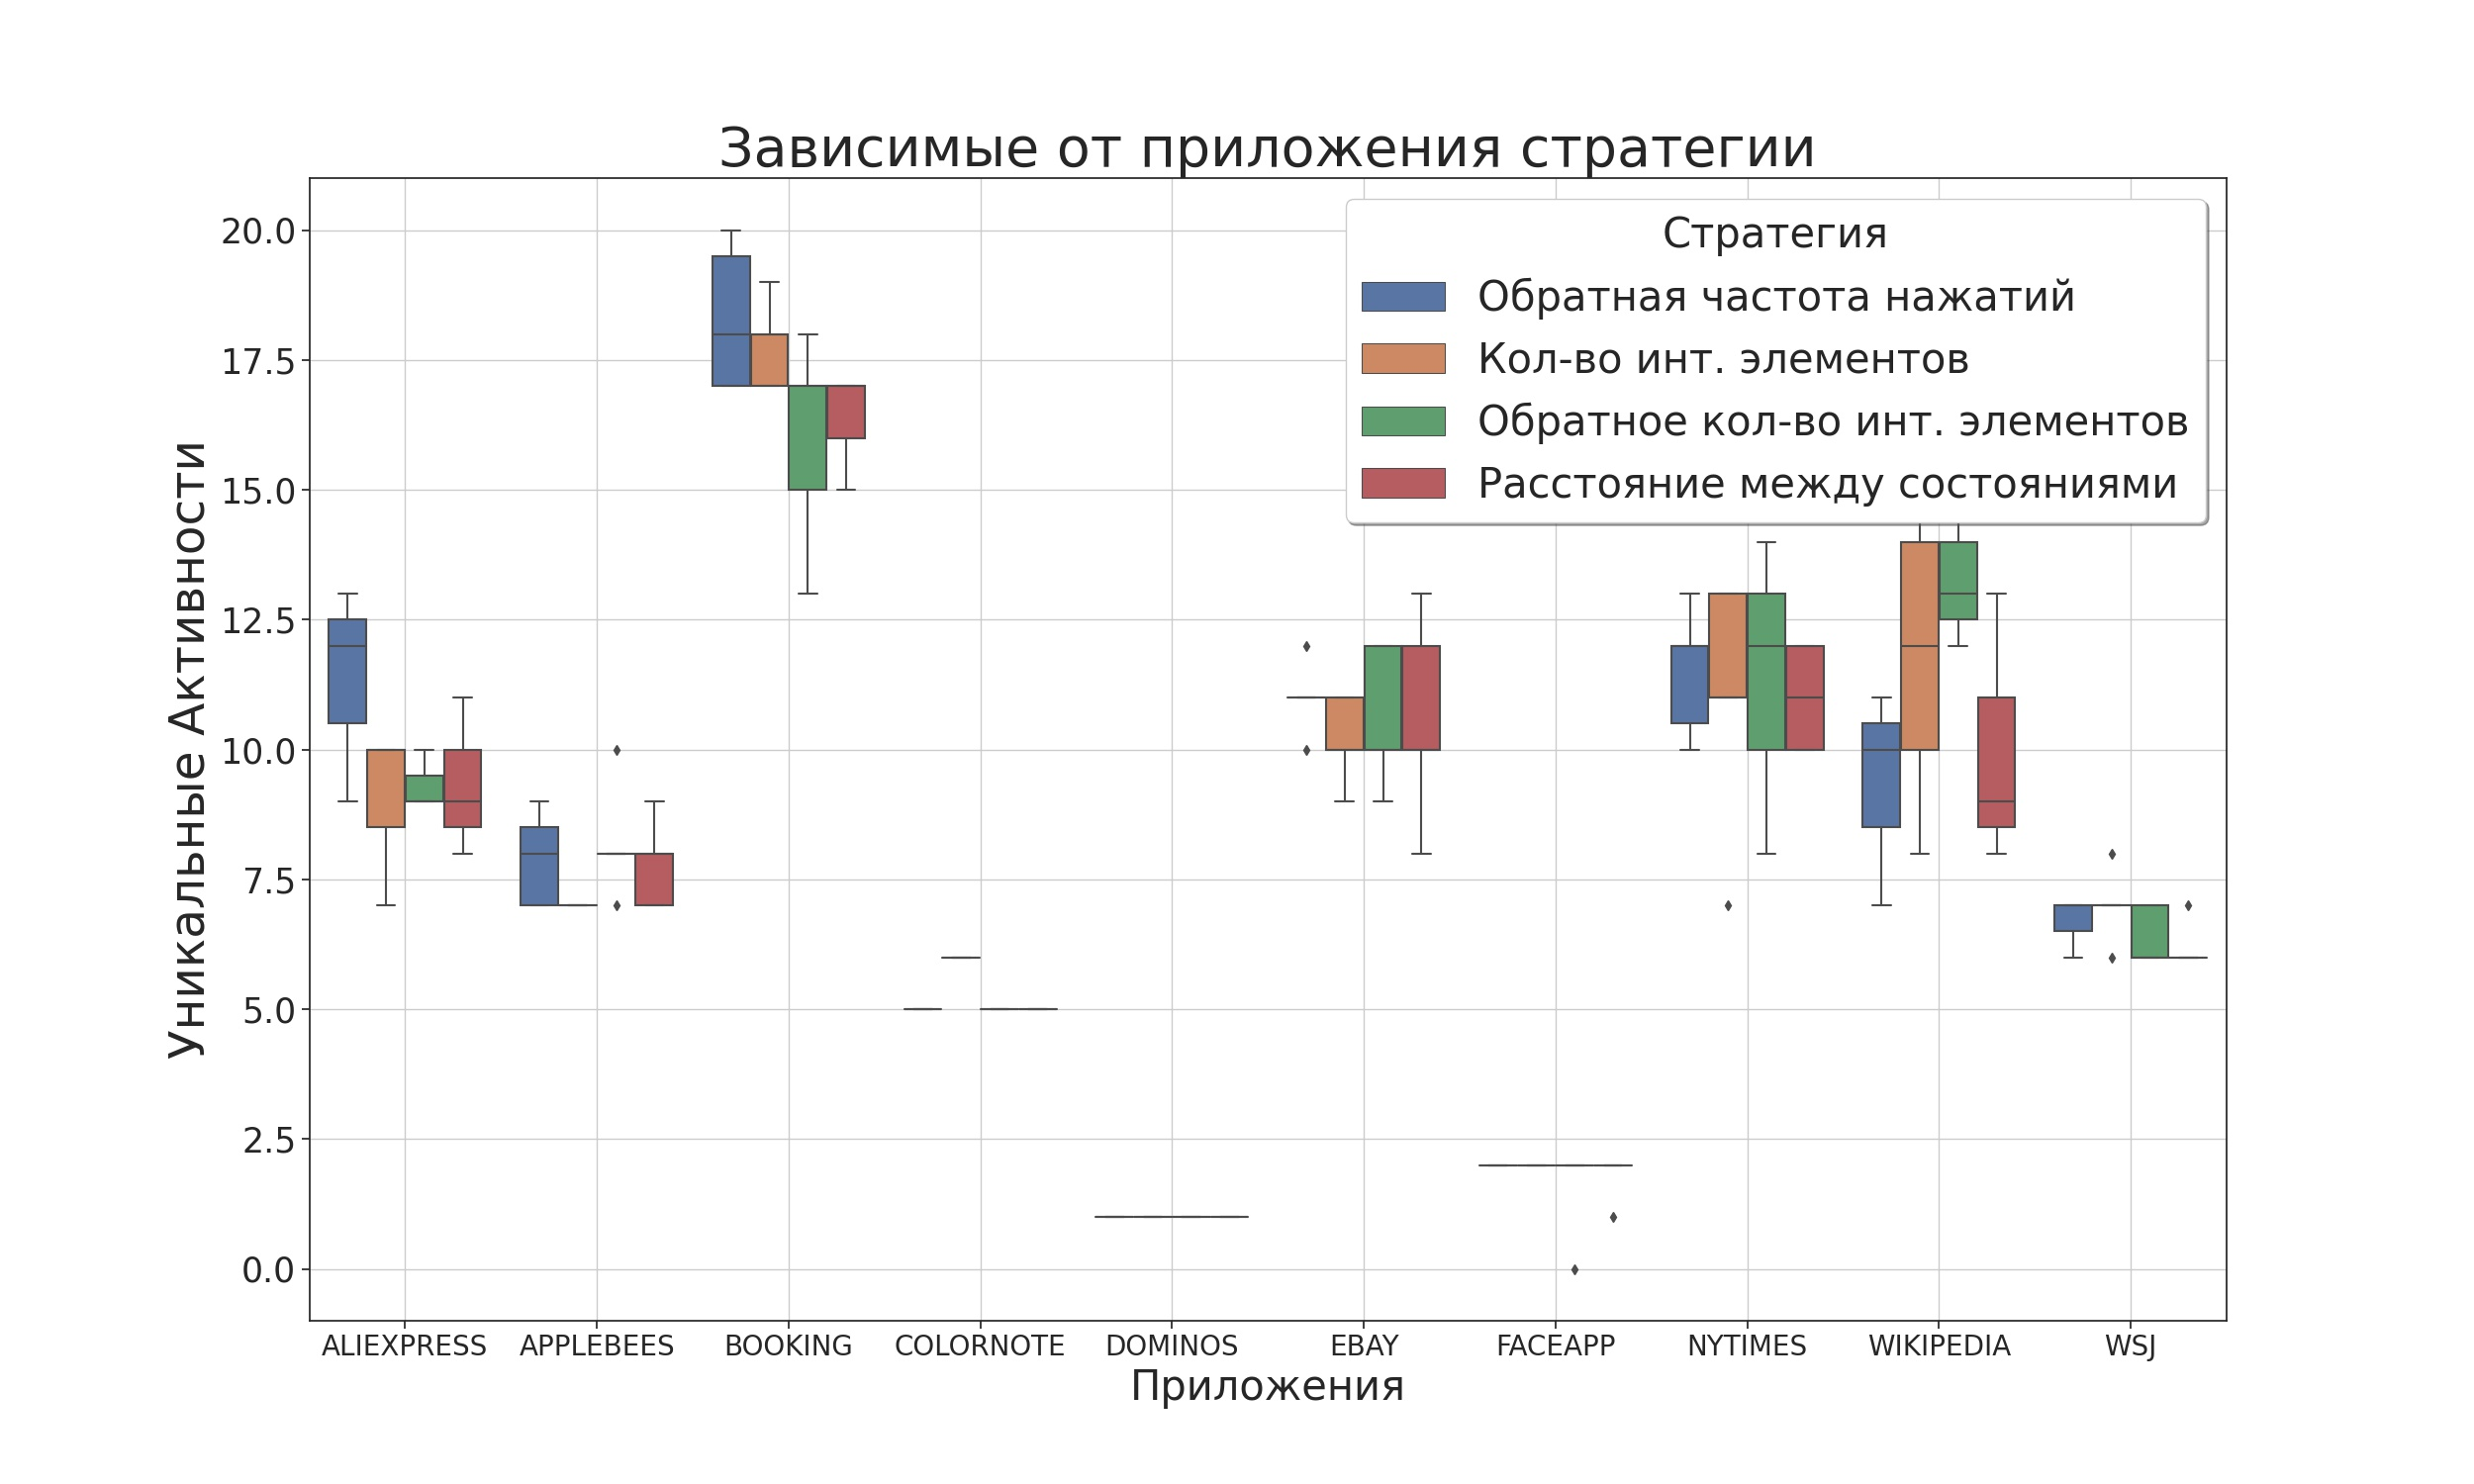
\includegraphics[width=400px]{activities_app_based.jpg}}
\caption{Зависимые от приложения стратегии тестирования.}
\label{app_based_picture}
\end{figure}

Если сравнивать между собой эвристики, которые использовались в функциях наград, то однозначного лидера выделить нельзя. С точки зрения метрики уникальных состояний, хороший результат показали награды за обратную частоту нажатий и обратное количество интерактивных элементов. При анализе результатов на приложении Wall Street Journal лучшей стратегией оказывается та, которая считает более ценные состояния с большим количеством интерактивных элементов. Функция наград с расстоянием между состояниями показала хороший результат на приложениях The New York Times и ColorNote, но все равно не стала лидером. Анализ показал, что близкие на внешний вид состояния могут иметь большое расстояние редактирования между деревьями этих состояний. Это не позволяет в полной мере использовать эту эвристику.

Для дальнейшего улучшения качества тестирования можно прибегнуть к приемам, которые используются во многих приложениях обучения с подкреплением и машинного обучения в целом. Рассмотрим применение некоторых из них в поставленной задаче.

\subsection{Эпсилон жадная стратегия}

Хорошей практикой обучения с подкреплением является добавление некоторой случайности на первых этапах обучения. Это позволяет агенту лучше изучить окружение, до того момента, пока алгоритм не обучится. Такая стратегия называется $\varepsilon$-жадная. Суть ее в том, что перед обучением задается число $\varepsilon$ близкое к единице, его роль -- определять вероятность, с которой агент будет делать случайное действие в текущем состоянии вместо того, чтобы соблюдать стратегию. По ходу обучения это число уменьшается, и через определенное количество времени агент действует только согласно стратегии. Такой подход позволяет на начальных этапах отдать предпочтение случайным действиям, нежели еще необученным алгоритмам. Этот метод позволяет производить более широкое исследование за счет смешивания двух алгоритмов: случайного и основанного на модели. Будем использовать в этом подходе функцию награды, описываемую формулой~(\ref{eq_reward}). Результаты тестирования этой стратегии приведены в Таблице~\ref{advansed_table}.


\subsection{Предобучение модели}\label{pretraining}

В теории машинного обучения принято разделять этапы обучения и использования модели. В поставленной задаче можно также воспользоваться этим правилом. Сначала на длительное время запустить изучение приложения для формирования Q-таблицы, а потом прочитать из файла готовую таблицу и на ней проводить тестирование. Важно понимать, что при формировании таблицы не нужно учитывать количество посещений каждого состояния, иначе на этапе тестирования будет сложно достичь часто посещаемых состояний.

В дополнение к предыдущему приему, можно выполнять тестирование в несколько эпизодов. Одна и та же Q-таблица будет переходить от одного эпизода к другому, а каждый эпизод будет начинать тестирование приложения с самого начала. Таким образом, во время тестирования можно имитировать несколько сессий взаимодействия пользователя, что должно повысить эффективность тестирования. Будем проводить тестирование в пять эпизодов, первые четыре из которых будут этапами обучения Q-таблицы, а последний этапом тестирования.

\begin{table}[h!]
    \centering
    \begin{tabular}{ | l | *{6}{>{\centering\arraybackslash}p{50} |}}
        \hline
        Приложения & 
        \multicolumn{2}{>{\centering\arraybackslash}p{110}|}{Эпсилон жадная стратегия} & 
        \multicolumn{2}{>{\centering\arraybackslash}p{110}|}{Предобученная модель} & 
        \multicolumn{2}{>{\centering\arraybackslash}p{110}|}{Предобученная модель с эпсилон жадной стратегией} \\
        \hline
        ALIEXPRESS &
        30 &
        13 & 
        \textbf{80} &
        16 & 
        63 & 
        \textbf{18} \\
        \hline
        APPLEBEES &
        35 &
        \textbf{9} & 
        \textbf{68} &
        8 & 
        63 & 
        8 \\
        \hline
        BOOKING &
        94 &
        17 & 
        \textbf{107} &
        15 & 
        97 & 
        \textbf{18} \\
        \hline
        COLORNOTE &
        130 &
        5 & 
        189 &
        5 & 
        \textbf{190} & 
        \textbf{6} \\
        \hline
        DOMINOS &
        37 &
        \textbf{1} & 
        \textbf{39} &
        \textbf{1} & 
        36 & 
        \textbf{1} \\
        \hline
        EBAY &
        \textbf{60} &
        \textbf{12} & 
        40 &
        9 & 
        34 & 
        11 \\
        \hline
        FACEAPP &
        63 &
        \textbf{2} & 
        \textbf{79} &
        \textbf{2} & 
        59 & 
        \textbf{2} \\
        \hline
        NYTIMES &
        \textbf{68} &
        \textbf{13} & 
        53 &
        10 & 
        60 & 
        11 \\
        \hline
        WIKIPEDIA &
        101 &
        13 & 
        139 &
        \textbf{14} & 
        \textbf{154} & 
        12 \\
        \hline
        WSJ &
        84 &
        8 & 
        117 &
        8 & 
        \textbf{134} & 
        \textbf{9} \\
        \hline
    \end{tabular}
    \caption{Улучшение стратегий тестирования. Метрика слева -- уникальные состояния, справа -- Активности.}
    \label{advansed_table}
\end{table}

На эпизодах обучения будем использовать функцию награды, равную числу интерактивных элементов в новом состоянии без учета количества посещений состояний. Таким образом удастся сформировать честную Q-таблицу, описывающую только количество интерактивных элементов. На эпизоде тестирования будем использовать обученную Q-таблицу, однако для предотвращения выбора одних и тех же действий теперь функция награды будет обратно пропорциональной количеству взаимодействий~(\ref{eq_reward}). Результаты этого подхода представлены в Таблице~\ref{advansed_table}.

Теперь попробуем добавить в эту стратегию элемент случайности. Объединим стратегию обучения в несколько эпизодов с эпсилон жадной стратегией. Будем использовать описанную ранее $\varepsilon$-жадную стратегию, однако в рамках одного эпизода значение $\varepsilon$ уменьшаться не будет. Уменьшение значения $\varepsilon$ будет происходить после эпизода. Таким образом, первый эпизод тестирования будет почти полностью случайным, а последний -- полностью подчиняться Q-learning стратегии. В итоге последний этап тестирования будет использовать обученную $\varepsilon$-жадной стратегией Q-таблицу. Результаты этого подхода представлены в Таблице~\ref{advansed_table}.


Результаты последних трех подходов либо превосходят все рассмотренные ранее стратегии, либо приближаются к лучшим результатам на них. Таким образом, предобучение модели и добавление в нее элемента случайности значимо повысило эффективность тестирования. Интересно заметить, что в обоих случайных подходах метрика Активностей выше, чем в обычной предобученной модели. Из этого следует, что случайность на первых этапах тестирования положительно сказывается на увеличении метрики Активностей.

\subsection{Анализ результатов}

Перед тем как сравнивать подходы обучения с подкреплением с другими инструментами тестирования мобильных приложений, проведем анализ полученных результатов и выберем подход, который производит наиболее эффективное тестирование.

Для начала стоит отметить, что стратегии, которые способны тестировать произвольное приложение, уступают тем, которые обучаются под единственное приложение. Этого следовало ожидать, так как реализация этих алгоритмов связана с рядом упрощений для совместимости с любым приложением.

Улучшение зависимых от приложения стратегий за счет добавления классических приемов машинного обучения приводит к увеличению метрик качества. Так три последние стратегии показали высокую производительность тестирования и превзошли почти все предыдущие стратегии. Можно заметить, что добавление случайности в алгоритм способствует повышению метрики Активности. Однако смешивание двух стратегий (предобучение и случайность) не позволило взять лучшее от каждого из подходов, и результат в среднем оказался ниже. Исключение составили три приложения: Wall Street Journal, ColorNote и Wikipedia. Однако их превосходство над стратегией с предобучением незначительное.

\begin{table}[h]
    \centering
    \begin{tabular}{ | l | *{8}{>{\centering\arraybackslash}p{37}|}}
        \hline
        Приложения & 
        \multicolumn{2}{>{\centering\arraybackslash}p{74}|}{Обратная частота нажатий} & 
        \multicolumn{2}{>{\centering\arraybackslash}p{74}|}{Обратное кол-во инт. элементов} &
        \multicolumn{2}{>{\centering\arraybackslash}p{74}|}{Предобученная модель} &
        \multicolumn{2}{>{\centering\arraybackslash}p{80}|}{Предобученная модель с эпсилон жадной стратегией} \\
        \hline
        ALIEXPRESS &
        37 &
        11 & 
        34 & 
        10 &
        \textbf{80} &
        16 & 
        63 & 
        \textbf{18} \\
        \hline
        APPLEBEES &
        32 &
        7 & 
        34 &
        \textbf{8} &
        \textbf{68} &
        \textbf{8} & 
        63 & 
        \textbf{8} \\
        \hline
        BOOKING &
        \textbf{116} &
        \textbf{18} &
        85 &
        16 &
        107 &
        15 & 
        97 & 
        \textbf{18} \\
        \hline
        COLORNOTE &
        142 &
        5 & 
        183 &
        5 &
        189 &
        5 & 
        \textbf{190} & 
        \textbf{6} \\
        \hline
        DOMINOS &
        35 &
        \textbf{1} & 
        30 &
        \textbf{1} &
        \textbf{39} &
        \textbf{1} & 
        36 & 
        \textbf{1} \\
        \hline
        EBAY &
        \textbf{67} &
        \textbf{11} & 
        40 &
        \textbf{11} &
        40 &
        9 & 
        34 & 
        \textbf{11} \\
        \hline
        FACEAPP &
        54 &
        \textbf{2} & 
        48 &
        \textbf{2} &
        \textbf{79} &
        \textbf{2} & 
        59 & 
        \textbf{2} \\
        \hline
        NYTIMES &
        \textbf{77} &
        11 & 
        49 &
        \textbf{12} &
        53 &
        10 & 
        60 & 
        11 \\
        \hline
        WIKIPEDIA &
        74 &
        9 & 
        95 &
        \textbf{14} &
        139 &
        \textbf{14} & 
        \textbf{154} & 
        12 \\
        \hline
        WSJ &
        96 &
        7 & 
        85 &
        7 &
        117 &
        8 & 
        \textbf{134} & 
        \textbf{9} \\
        \hline
    \end{tabular}
    
    \caption{Сравнение лучших стратегий тестирования. Метрика слева -- уникальные состояния, справа -- Активности.}
    \label{results_table}
\end{table}

В результате анализа двух метрик качества на десяти приложениях можно выделить четыре лидирующих подхода: подход с наградой за обратную частоту нажатий (пункт \ref{events_count}), подход с наградой за обратное количество интерактивных элементов (пункт \ref{possible_events}), подход с предобучением Q-таблицы (пункт \ref{pretraining}), подход с предобучением и случайностью (пункт \ref{pretraining}). Результаты экспериментов этих стратегий можно увидеть в таблице~\ref{results_table}. Сравнивая их метрики качества, можно заметить, что подход с предобучением Q-таблицы ведет себя наиболее стабильно. Даже если его результаты ниже конкурентов, они все равно довольно близки к лидирующим и высоки в сравнении с другими алгоритмами. Таким образом, лучшим из разработанных в данной работе методов является метод с предобучением таблицы. Именно он будет сравниваться с другим инструментом тестирования в следующем пункте.

\subsection{Сравнение с Humanoid}

В предыдущем пункте удалось выделить лидирующий Q-learning подход. Будем использовать его для сравнения подходов обучения с подкреплением с современным подходом к тестированию, основанном на глубоких нейронных сетях Humanoid~\cite{li2019deep}. Humanoid обучается таким образом, чтобы максимально соответствовать человеческому поведению.


\begin{figure}[h]
\subfloat[Метрика: состояния.]{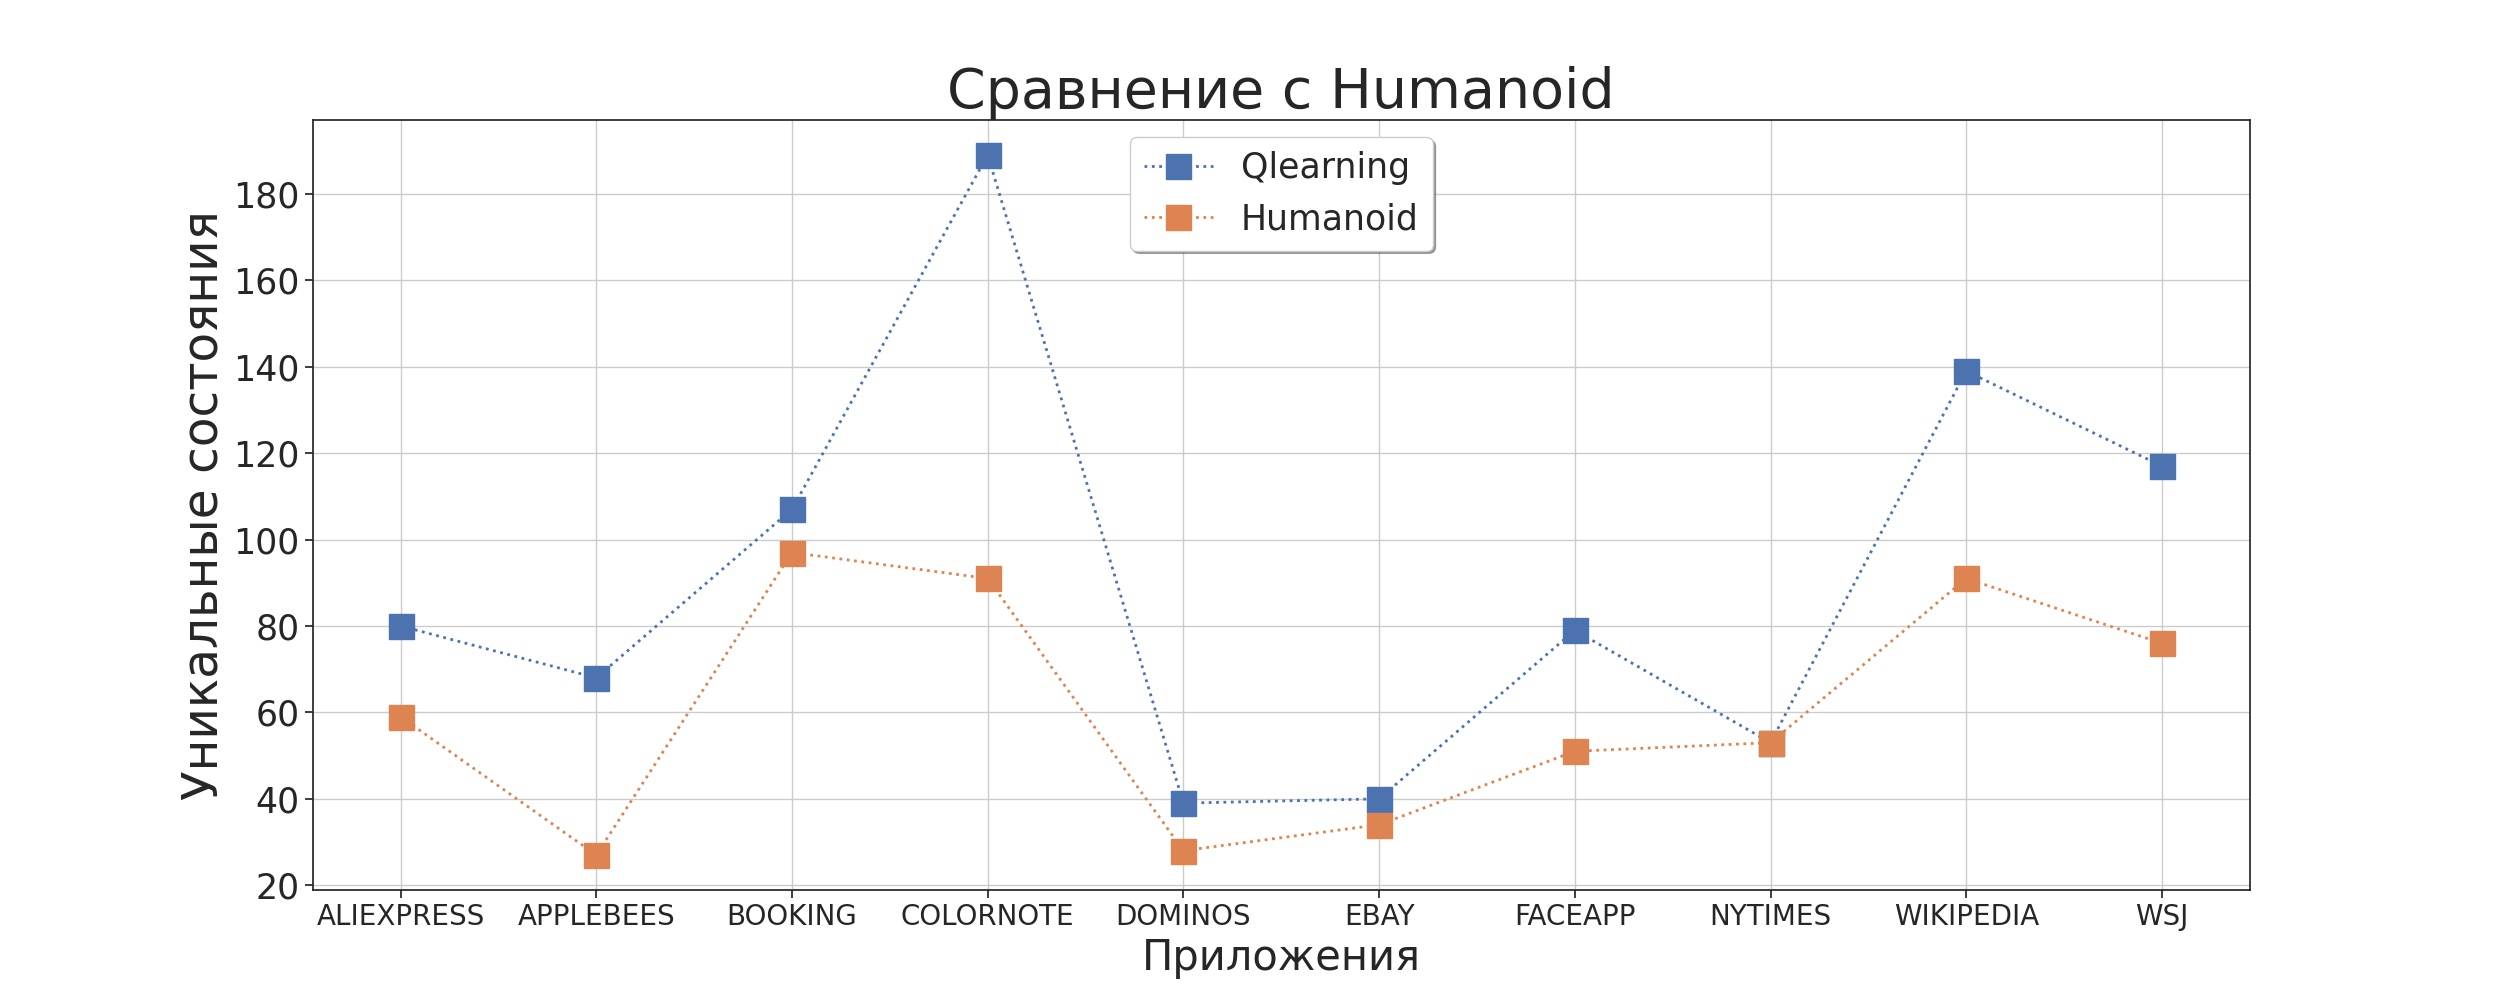
\includegraphics[width=450px]{states_humanoid.jpg}} \\
\subfloat[Метрика: Активности.]{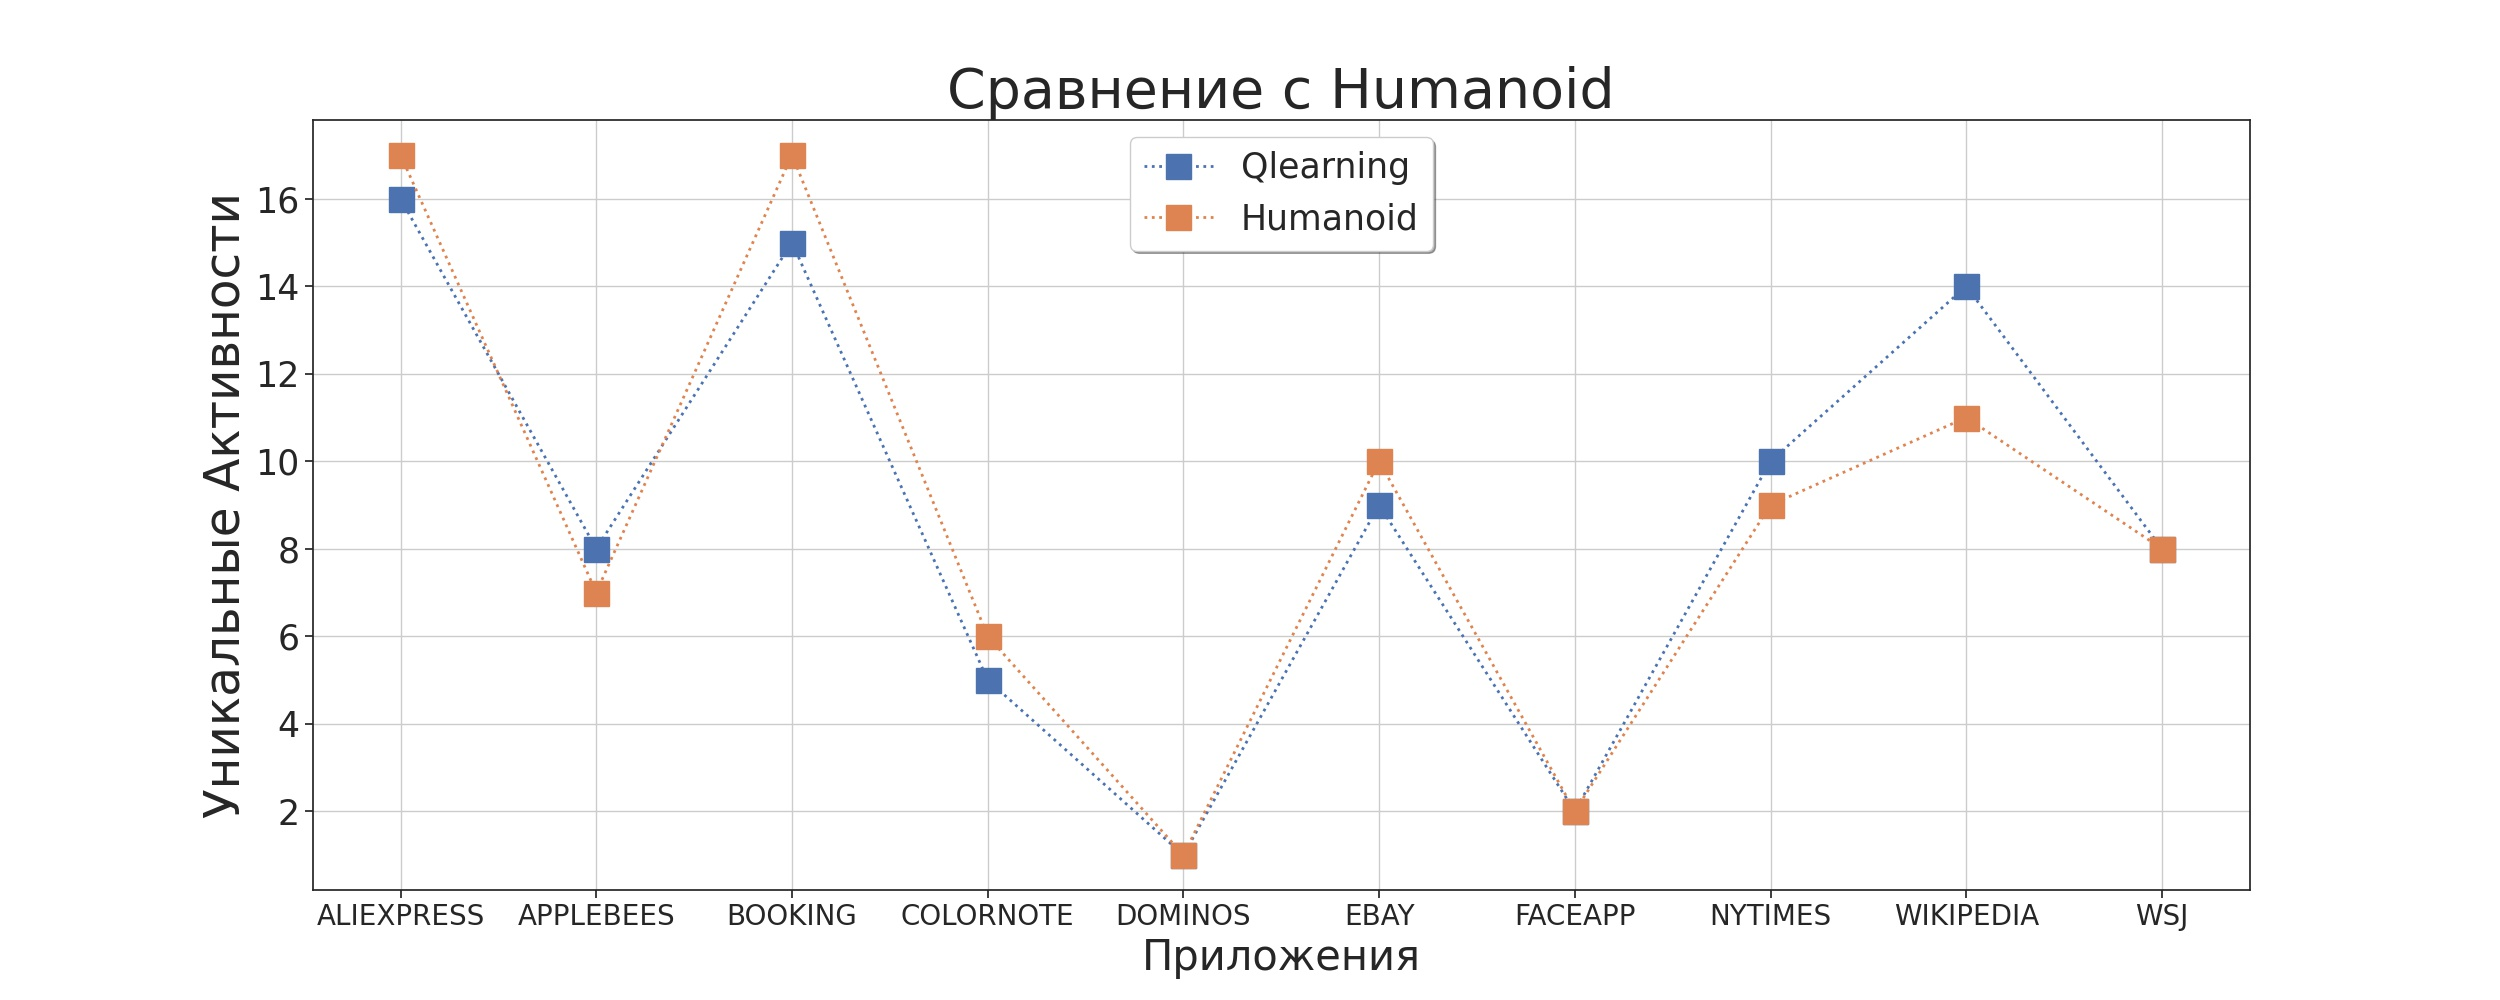
\includegraphics[width=450px]{activities_humanoid.jpg}}
\caption{Сравнение Q-learnign подхода с Humanoid подходом.}
\label{Humanoid}
\end{figure}

Эксперименты с инструментом Humanoid будем проводить при тех же условиях, что использовались для других экспериментов (5 запусков по 12 минут). Результаты сравнения можно видеть на Рис.~\ref{Humanoid}. Подход обучения с подкреплением с предобучением Q-таблицы превзошел инструмент тестирования Humanoid по метрике уникальных состояний. Если сравнивать два подхода по метрике уникальных Активностей, то ни один из подходов значимо не превосходит другой. % Исследование и построение решения задачи
\section{Описание практической части}
\label{sec:Chapter4} \index{Chapter4}

Для реализации алгоритмов в работе использовался язык программирования Python. Основной причиной в пользу выбора этого языка был тот факт, что тестирующая система DroidBot написана на Python, и для удобного внедрения было принято решение все алгоритмы писать на этом языке. Также Python удобен тем, что предоставляет обширную стандартную библиотеку и множество дополнительных модулей. Это позволяет вести разработку с большой скоростью, без реализации классических алгоритмов.

Реализация большинства подходов ограничивалась стандартной библиотекой  Python. Однако, для некоторых алгоритмов приходилось использовать библиотеки для обработки и визуализации данных: numpy, pandas, matplotlib. Так же для подсчета расстояния редактирования графов была подключена библиотека zss, а для реализации сверточной нейронной сети использовалась библиотека keras.

Все алгоритмы тестирования встраивались в тестирующую систему DroidBot~\cite{li2017droidbot} (Рис.~\ref{InteractionScheme}). Тестирующая система использовалась для того, чтобы основное внимание при решении задачи уделялось реализации алгоритмов тестирования, а не проблемам взаимодействия с устройством. DroidBot состоит из нескольких основных компонентов: \texttt{Device}, \texttt{DeviceState}, \texttt{Environment}, \texttt{InputEvent}, \texttt{InputPolicy}. Все они являются классами языка Python. Класс \texttt{Device} описывает взаимодействия которые происходят с устройством: установка/удаление приложения, получение текущего состояния, получение метаинформации о состоянии, воспроизведение нажатий. Как отмечалось ранее, эти действия происходят через низкоуровневый инструмент Android Debug Bridge. Класс \texttt{DeviceState} отвечает за представление состояния на устройстве, через него также можно получить список интерактивных элементов и возможные взаимодействия с ними. В классе \texttt{Environment} происходит основное взаимодействие тестирующего алгоритма и устройства. В нем задаются настройки тестирования и сохраняются результаты. \texttt{InputEvent} представляет из себя базовый класс для представления произвольного взаимодействия с устройством. Все жесты наследуются от этого класса.

Самым важным для этой работы классом в системе тестирования DroidBot является класс \texttt{InputPolicy}. Это базовый класс всех стратегий тестирования. Для генерации нажатия вызывается метод этого класса \texttt{generate\_event}, который получает на вход обработанное состояние приложения и возвращает действие, которое нужно воспроизвести на устройстве. Это и есть основный цикл, который проходят алгоритмы тестирования.

\begin{figure}[h]
\center{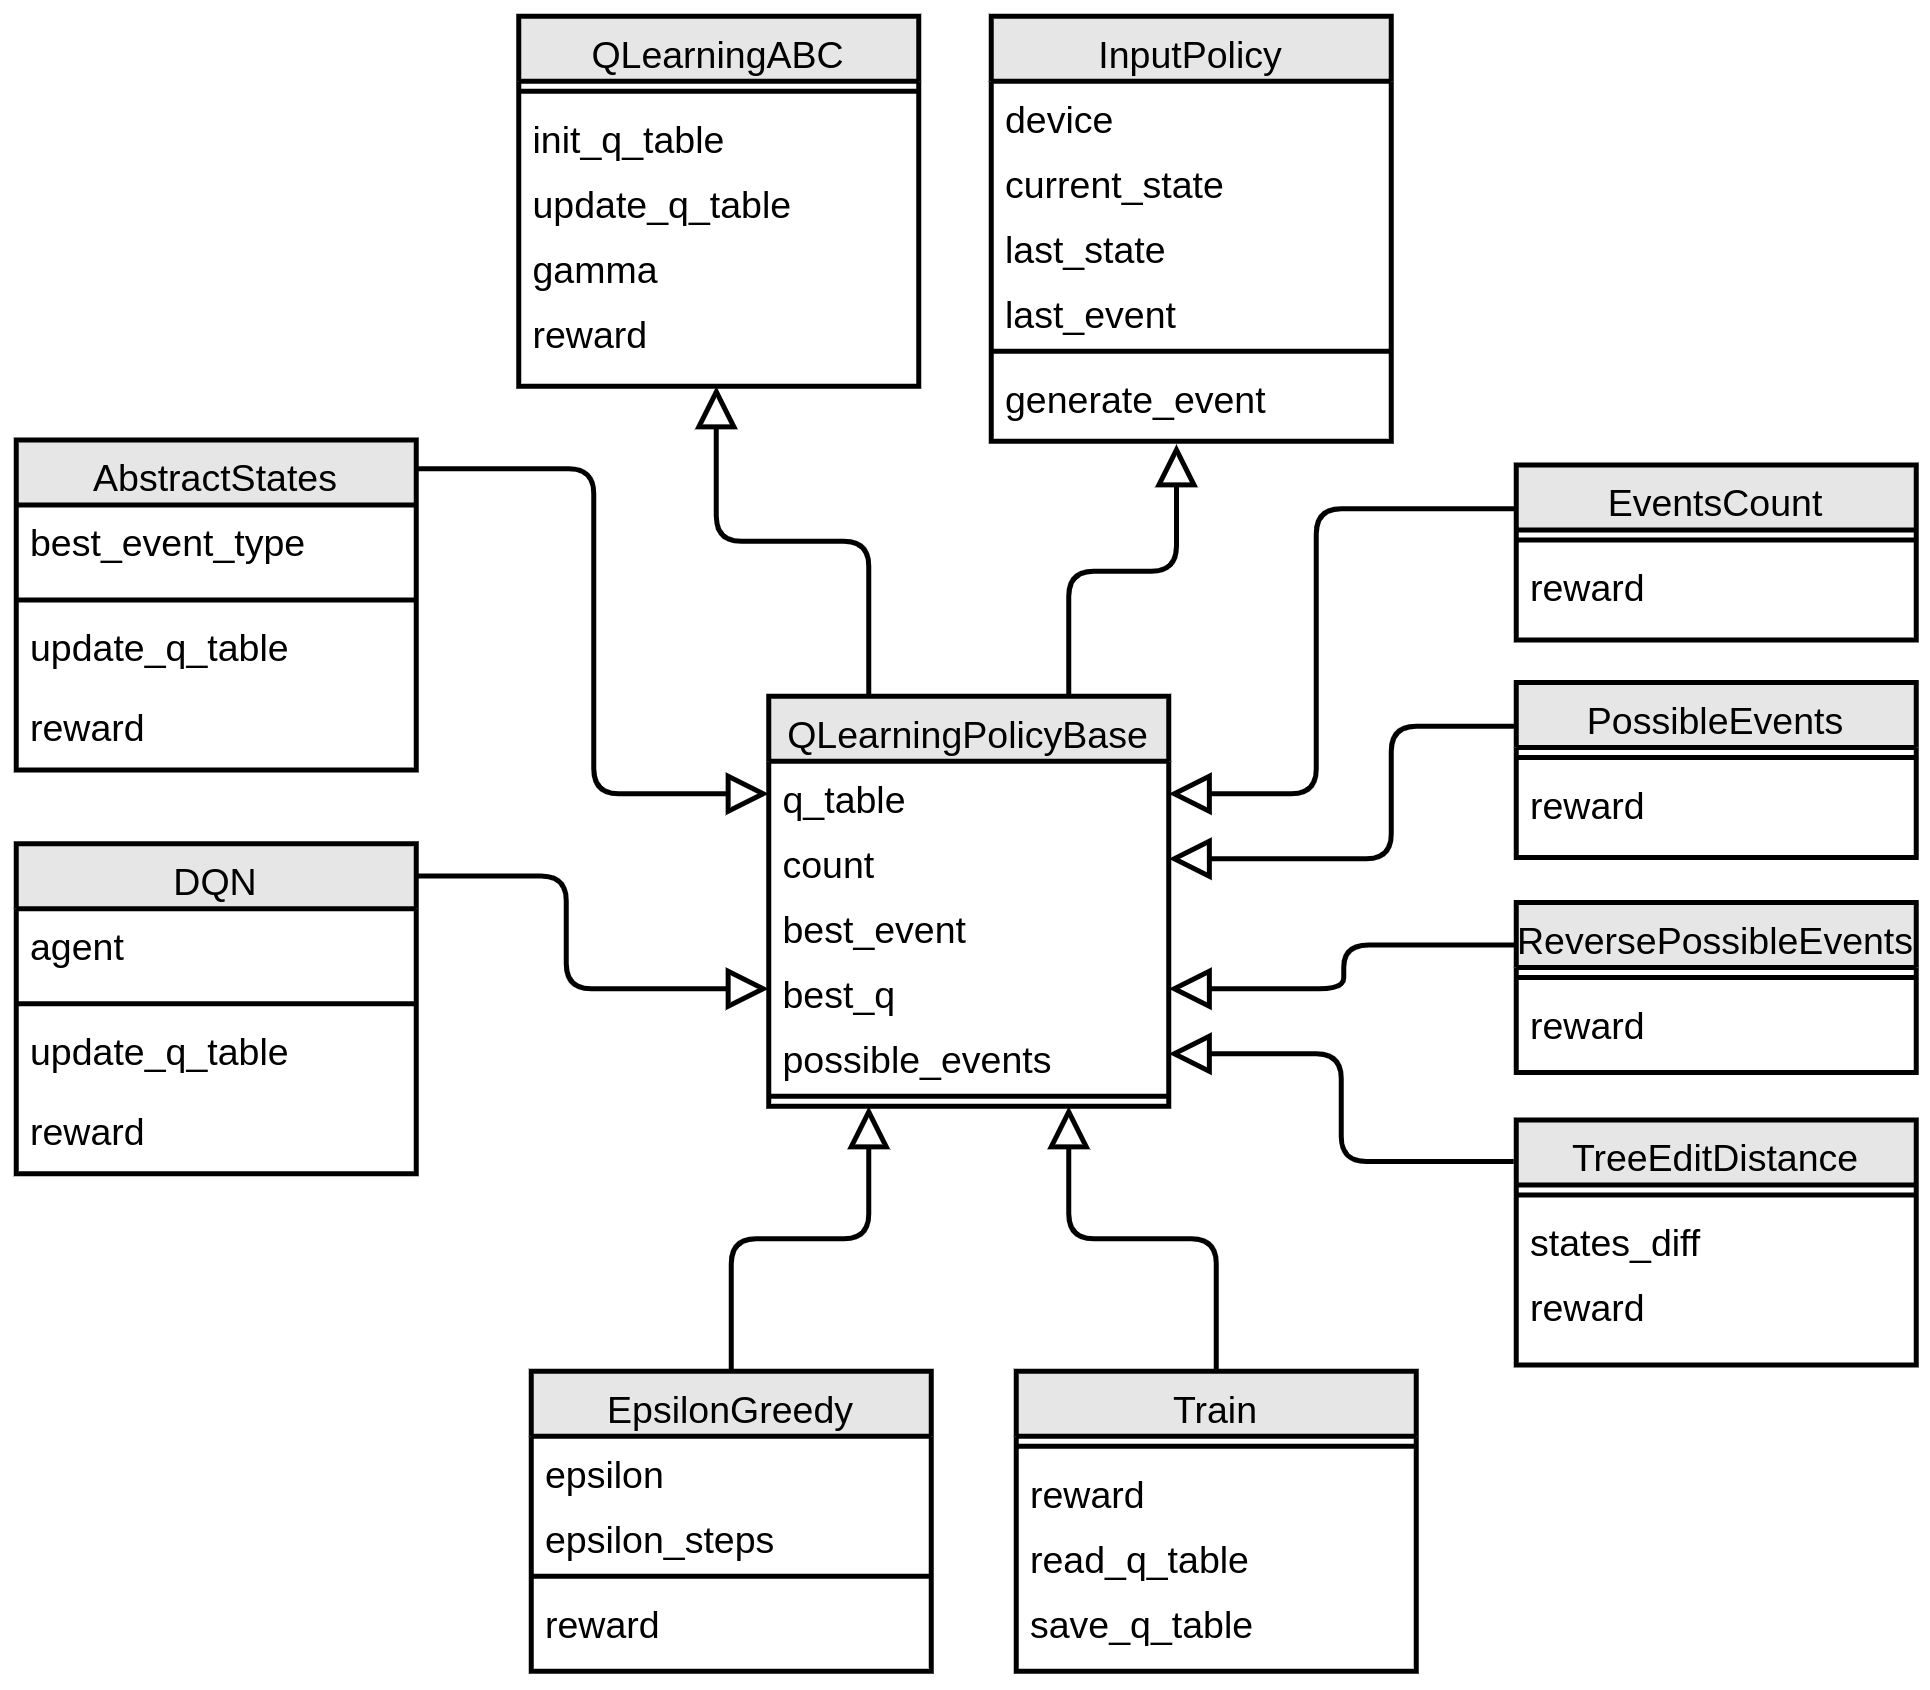
\includegraphics[width=450px]{UMLdiagram.png}}
\caption{UML диаграмма классов стратегий тестирования.}
\label{UML}
\end{figure}

Алгоритмы обучения с подкреплением реализовывались отдельными классами. Их UML диаграмма представлена на Рис.~\ref{UML}. На этой диаграмме можно увидеть два базовых класса: \texttt{QLearningABC} и \texttt{InputPolicy}. Первый содержит абстрактные методы, которые должны быть перегружены в любой Q-learning стратегии, второй -- весь необходимый функционал для встраивания стратегии в DroidBot. Класс \texttt{QLearningPolicyBase} наследует эти два класса и описывает базовую функциональность произвольного Q-learning алгоритма: создание таблицы, подсчет числа взаимодействий, алгоритмы поиска максимального Q-значения и т. д. Все остальные классы на UML диаграмме являются реализацией определенной стратегии из предыдущей главы и наследуются от \texttt{OLearningBase}. 

Все алгоритмы высокоуровнево можно описать одной и той же последовательностью действий:

\begin{enumerate}

\item Ожидание запроса для генерации действия (\texttt{generate\_event})

\item Получение запроса вместе с текущим состоянием (\texttt{generate\_event\_based\_on\_utg})

\item Получение списка возможных взаимодействия в текущем состоянии (\texttt{possible\_events})

\item Поиск лучшего действия согласно Q-таблице (\texttt{update\_best})

\item Обновление Q-значения для предыдущего состояния и действия (\texttt{update\_q\_table})

\item Возврат лучшего действия для воспроизведения на устройстве (\texttt{best\_event})

\end{enumerate} % Описание Экспериментальной части
\section{Заключение}
\label{sec:Chapter5} \index{Chapter5}

В данной работе были исследованы современные методы динамического тестирования мобильных приложений через взаимодействие с графическим интерфейсом. Основное внимание было уделено изучению перспективных подходов, основанных на алгоритмах обучения с подкреплением.

В ходе работы были изучены основы функционирования алгоритмов обучения с подкреплением и популярный подход Q-learning. Были реализованы и протестированы существующие подходы для решения поставленной задачи. Также проводились эксперименты с изменением и улучшением существующих подходов, путем добавления некоторых эвристик, в том числе основанные на сверточных нейронных сетях. Были реализованы подходы способные тестировать целый набор приложений, используя одну модель обучения с подкреплением для всех приложений. Для повышения качества тестирования были реализованы алгоритмы, способные тестировать единственное приложение, под которое они обучаются. Также проводились эксперименты по внедрению идей из классического машинного обучения.

Результаты показывают, что подходы, предназначенные для тестирования одного приложения, превосходят обобщенные модели, способные тестировать набор приложений. Также добавление логичных эвристик даже в самые простые реализации способно повысить производительность тестирования. Можно сделать вывод, что не все современные подходы способны удовлетворять требованиям практического применения алгоритмов. В результате экспериментов удалось выделить алгоритм, основанный на предварительном обучении. Он значимо превосходит эвристические предположения.

В результате сравнения с современным подходом к тестированию Humanoid, лучший из методов обучения с подкреплением оказался существенно эффективней в рамках поставленной задачи.

Результаты этой работы будут использованы в промышленном продукте, разрабатываемом в Институте системного программирования им. В.П. Иванникова РАН. В перспективе можно рассмотреть влияние альтернативного представления состояний приложения. В том числе представление на основе графовых вложений. % Заключение

\nocite{*}
\bibliographystyle{gost71u} % Для соответствия требованиям об оформлении списка литературы
\bibliography{references}

% \section*{Приложение}
\addcontentsline{toc}{section}{Приложение}
\label{sec:Apendix} \index{Apendix}

 

\end{document}
